\documentclass{article}
\usepackage[utf8]{inputenc}

\title{\textbf{TMC1}:
Machine Learning for drug target identification}
\author{David Narganes-Carlon}
\date{25th January 2019}
\usepackage{mathtools}          % mathematics notation
\usepackage{graphicx}           % manipulation of images
\usepackage{booktabs}           % tables
\usepackage{multicol}           % multiple columns
\usepackage{float}              % pictures in place
\usepackage{hyperref}
\usepackage{amssymb}
\usepackage{listings}
\usepackage{subfig}
\usepackage{array}
\usepackage[font=small]{caption}
\usepackage[a4paper,
            bindingoffset=0.2in,
            left=1.9cm,
            right=1.9cm,
            top=2cm,
            bottom=2cm,
            footskip=.25in]{geometry}

\hypersetup{
    colorlinks=true,
    citecolor=red,
    linkcolor=blue,
    urlcolor=blue,
}

\usepackage{color}
\definecolor{codegreen}{rgb}{0,0.5,0}
\definecolor{pink}{rgb}{1,0.07,0.57}
\definecolor{codegray}{rgb}{0.4,0.4,0.5}
\definecolor{codepurple}{rgb}{0.58,0,0.82}
\definecolor{backcolour}{rgb}{0.95,0.95,1}
 
\lstdefinestyle{mystyle}{
    backgroundcolor=\color{backcolour},   
    commentstyle=\color{blue},
    keywordstyle=\color{pink},
    stringstyle=\color{codepurple},
    basicstyle=\footnotesize,
    breakatwhitespace=false,         
    breaklines=true,                 
    captionpos=b,                    
    keepspaces=true,                 
    showspaces=false,                
    showstringspaces=false,
    showtabs=false,                  
    tabsize=2
}
\lstset{style=mystyle}

\begin{document}
\maketitle
\tableofcontents
\newpage

\section{Introduction}
Traditionally, in drug discovery, target identification to develop novel agents for any given disease is carried out on a case-by-case basis. In this model, individual scientists act as project champions for targets based on available literature and local expertise. Nevertheless   drug discovery is extremely costly and failure-prone \cite{ferrero2017}. Nevertheless:

\begin{enumerate}
    
    \item With increasing publication rates, it is becoming impossible to maintain an overview over an increasingly vast scientific literature. The large quantity not just biomedical research literature but also orthogonal perspectives continually being produced renders it impossible for individual researchers and corporations to keep up to date \cite{brown2018}. Therefore, the development of \textbf{alert systems for emerging targets and trends in the literature} at a genome scale is of prime importance in the pharmaceutical sector.
    
    \item In recent years a wealth of biological data from multiple domains has become available in \textbf{public data repositories} \cite{brown2018}. A firm integration of this extensive and extremely valuable corpus of scientific literature is necessary for a rapid generation of new, high-quality hypothesis for drug discovery without the need of human intervention \cite{ferrero2017, brown2018}.
    
    \item Drug discovery is extremely costly and failure-prone \cite{ferrero2017}. As the cost of successful drug development continues to increase, the productivity of the industry as a whole in launching new drugs remains flat \cite{brown2018}.

\end{enumerate}

\noindent
Hence, both putative target and topic prioritisation in drug discovery (i) is of paramount importance to maximise the chances of success in clinic \cite{ferrero2017} and (ii) ensures a sustainable business in the long term \cite{ferrero2017}.

\subsection{Proposed approach}
Based on the \href{https://goo.gl/QrfdfY}{initial proposal}, this PhD iCASE will focus on the development of an innovative integrated resource which uses machine learning algorithms to exploit a newly generated semantic repository to facilitate a systematic genome scale ranking of potential targets in the areas of type 2 diabetes, non-alcoholic steatohepatitis (NASH) and metabolic syndrome: putative therapeutic target prioritisation (PTTP).

In order to do so, the student divided the project into two subparts:
\begin{enumerate}
\item Develop machine learning methods to create an alert system for emerging targets from PubMed 2019 version
\item Develop a comprehension about the publicly available biomedical resources to create an integrated resource for putative therapeutic target prioritisation (PTTP) for the next months of the project (please see Project Description: Machine Learning for drug target identification also presented to this Tribunal Committee)
\end{enumerate}
\newpage

\section{Literature Review}
\label{section:lit_review}

Linking human genes to the diseases in which they are involved lies at the very heart in the drug discovery process \cite{DISEASES2015,ferrero2017,brown2018}. Such links can be made through a variety of different types of studies (e.g. Mendelian and complex diseases, GWAS, somatic mutation frequencies, transcriptomics, epigenetics and proteomics studies, detailed molecular biology studies of individual proteins, etc.) and, therefore, is important to develop an integration of those sources to comprehend the mechanisms underlying the cause of disease states and prevent or treat such conditions \cite{DISEASES2015,ferrero2017,brown2018}. The main focus of the literature review is for the student to gain an understanding of the publicly available biomedical resources. Nonetheless, (i) each individual resource has a specific scope and can only shed light on a limited set of scientific questions \cite{brown2018,DISEASES2015}, (ii) all relevant data is not collected on a single place \cite{brown2018,DisGeNET2015}, and (iii) the availability and interoperability of open and fully contextualised data sets remains a key issue in the full development and application of big data workflows to early drug discovery hypothesis generation \cite{brown2018}. However, there is a vast amount of GDAs in the biomedical literature and, therefore, the starting point of the \emph{practical} point of this PhD was to work with the biggest biomedical archive, PubMed version 2018 (see Section \ref{section:disambiguation}).

Several resources were developed to provide information on GDAs by integrating multiple data sources: (i) DrugBank \cite{drugbank2008}, (ii) the Therapeutic Target Database \cite{ttd2018}, (iii) STITCH \cite{stitch42014}, (iv) PharmaGKB \cite{pharmaGSK2012}, and SuperTarget \cite{superTarget2012}.

The emphasis of these databases is on the known and predicted interactions between the clinical trial drugs and their targets, how drug effects on targets are propagated through their corresponding pathways, their relationships to diseases, adverse events of drugs and pharmacogenomics \cite{brown2018}. Nevertheless, they do not provide a PTTP. There has been some attempts to develop a more systematic approach for PTTP (see Table \ref{tab:related_work}).

\begin{table}[H]
\centering
    \begin{tabular}{c|c|c}
      GDA Initiative & Section & Citation \\
      \hline
      
      \href{https://goo.gl/ewnpWZ}{DisGeNET} & \ref{subsec:DisGeNET} & \cite{DisGeNET2015} \\
      
      \href{https://goo.gl/KGQsd9}{DISEASES} & \ref{subsec:DISEASES} & \cite{DISEASES2015} \\
      
      \href{https://goo.gl/dPWHNY}{PHAROS} &  \ref{subsec:pharos} & \cite{pharos2016} \\
      
      \href{https://goo.gl/eQ667p}{Open Targets} & \ref{subsec:ot} & \cite{koscielny2016} \\
      
      \end{tabular}
\caption{PTTP initiatives, section in the report, and publication \label{tab:related_work}}
\end{table}

% DISGENET
\subsection{DisGeNET} \label{subsec:DisGeNET}
\href{https://goo.gl/ewnpWZ}{DisGeNET} is a discovery platform designed to address questions concerning the genetic underpinning of human diseases by analysing GDAs \cite{DisGeNET2015}. DisGeNET is organised according to the type and level of curation (see Table \ref{tab:disgenet_data} and \href{https://goo.gl/ntXTjX}{DisGeNET statistics}.

\begin{table}[H]
    \centering
    \resizebox{\textwidth}{!}{
    \begin{tabular}{c|c|c|c|c|c}
    Source & Type & Genes & Diseases & GDAs & Description \\
    \hline
    
    \href{https://goo.gl/XtufGc}{UniProt} &
    C & 19027 & 6303 & 20722 &
    Curated protein functional information \cite{uniprot2017} \\
    
    \href{https://goo.gl/aTyMBE}{CTDh} &
    C & 7787 & 4929 & 25975 &
    Environmental chemicals, genes and diseases \cite{ctd2017} \\
    
    \href{https://goo.gl/89TfbR}{ClinVar} &
    C & 45546 & 5639 & 54888 &
    Genetic human variants and diseases \cite{clinvar2016} \\
    
    \href{https://goo.gl/KxxD8Y}{GWASC} &
    C & 15790 & 610 & 20719 &
    GWAS catalog \cite{gwasCatalog2017} \\
    
    \href{https://goo.gl/hUkKLf}{Orphanet} &
    C & 2661 & 6702 & 97547 &
    Rare disorders, genes, and orphan drugs \cite{orphanet2012} \\

    \href{https://goo.gl/mgFWK4}{PsyGeNET} &
    C & 1546 & 112 & 3757 &
    Psychiatric GDAs \cite{PsyGeNET2015} \\

    \href{https://goo.gl/gYHKF3}{HPO} &
    C & 2661 & 6702 & 97547 &
    Phenotypic vocabulary for human diseases \cite{humanPhenotypeOntology2014} \\
    
    \href{https://goo.gl/aTyMBE}{CTDr} &
    M & 22 & 13 & 31 &
    CTD for \textit{Rattus Norvergicus} \cite{ctd2017} \\
    
    \href{https://goo.gl/aTyMBE}{CTDm} &
    M & 22 & 13 & 31 &
    CTD for \textit{Mus Musculus} \cite{ctd2017} \\
    
    \href{https://goo.gl/zc52JW}{RGD} &
    M & 1076 & 629 & 4291 &
    Genomic and disease data of \textit{R Norvegicus} \cite{rgd2015} \\
    
    \href{https://goo.gl/iTNmRx}{MGD} &
    M & 1464 & 1323 & 1994 &
    Genomic and disease data of \textit{M Musculus} \cite{mgd2015} \\
    
    \href{https://goo.gl/y3keCN}{GAD} &
    L & 13318 & 3099 & 63063 &
    GWAS repository \cite{gad2004}. Retired on 09/01/2014 \\
    
    \href{https://goo.gl/szDDw6}{LHGDN} &
    L & 5941 & 1799 & 31468 &
    Semantic ML extraction of GDAs \cite{bundschus2008} \\
    
    \href{https://goo.gl/4Yau27}{BeFree}* &
    L & 35392 & 16274 & 453574 &
    Biomed Name-Entity Recogniser of GDAs \cite{bravo2015} \\
    
    Total &  & 100076 & 29539 & 696707 \\
    
    \end{tabular}}
    \caption{Original data sources used by DisGeNET v5.0 \cite{DisGeNET2015}, type (\textbf{C} for curated data sources, \textbf{M} for Animal model data sources, and \textbf{L} for literature evidence sources), number of genes or gene variants, number of diseases or phenotypes, number of Gene--Disease Associations (GDAs or VDAs) and brief description. Information obtained from
    \href{https://goo.gl/ntXTjX}{DisGeNET statistics} \label{tab:disgenet_data}}
\end{table}

% DISEASES
\subsection{DISEASES}
\label{subsec:DISEASES}
\href{https://goo.gl/KGQsd9}{DISEASES} integrates evidence on GDAs from (i) automatic text mining, (ii) manually curated literature, (iii) cancer mutation data, and (iv) GWAS \cite{DISEASES2015}. They further integrate all evidence data and define confidence scores that facilitate comparison of the different types and sources of evidence \cite{DISEASES2015}.

They use a Named Entity Recogniser (NER) that maps diseases in Medline abstracts to the \href{http://disease-ontology.org/}{Disease Ontology} \cite{schriml2012} in two processes: (i) namely recognition and (ii) normalization (also known as identification, mapping, or grounding).

DISEASES integrates the GDAs extracted from automatic text mining with evidence from databases with permissive licenses, namely manually curated associations (see Table \ref{tab:diseases_data}).
\begin{table}[H]
\centering
    \begin{tabular}{c|c}
         Source & Description  \\
         \hline
         \href{https://goo.gl/gnQSYt}{GHR} & Genetic variation and diseases at NIH*\\
         \href{https://goo.gl/d2PhpC}{UniProtKB} & Curated protein functional data \cite{uniprot2017} \\
         \href{https://goo.gl/hYjVeR}{DistiLD} & GWAS linked to ICD-10 codes \cite{palleja2011} \\
         \href{https://goo.gl/qcY8qo}{COSMIC} & Somatic mutation cancer data \cite{cosmic2017}
    \end{tabular}
    \caption{Data sources used by DISEASES \cite{DISEASES2015} \label{tab:diseases_data}}
\end{table}

% PHAROS
\subsection{PHAROS}
\label{subsec:pharos}

The \href{https://druggablegenome.net/}{Illuminating the Druggable Genome} (IDG) was initially motivated to shed light to 1700 targets from four privileged drug target families \cite{santos2016}: G-Protein Coupled Receptors (GPCRs), kinases, ion channels, and nuclear receptors \cite{pharos2016}. Nevertheless, IDG is moving beyond those 4 families and now considers all 20k human coding genes \cite{pharos2016} based on phylogenecity, function, target development level, disease association, tissue expression, chemical ligand and substrate characteristics, and target-family specific characteristics. They developed the \href{http://drugtargetontology.org}{Drug Target Ontology (DTO)} \cite{lin2017}, also available on \href{http://github.com/DrugTargetOntology/DTO}{GitHub} and the \href{http://bioportal.bioontology.org/ontologies/DTO}{NCBO Bioportal}.

The \href{http://juniper.health.unm.edu/tcrd/}{Target Central Resource Database (TCRD)} is the central resource behind the Illuminating the Druggable Genome Knowledge Management Center (IDG-KMC) and can be downladed  \href{http://juniper.health.unm.edu/tcrd/download/}{here}. A list of the datasources used can be found \href{http://targetcentral.ws/Pharos}{here}.

Among PHAROS resources is \href{http://amp.pharm.mssm.edu/Harmonizome/about}{Harmonizome}, that aims to integrate a wide collection of public, disjoint datasets from multiple, internationally recognised datasets (n=114 in October 2018) from 66 different databases that gather information about genomics, epigenetics, transcriptomics, metabolomics, cell lines, diseases, physical interactions, drugs, and curated biomedical literature about mammalian cells \cite{harmonizome2016}. Actualised statistics of Harmonizome can be found \href{http://amp.pharm.mssm.edu/Harmonizome/about}{elsewhere}. One of their main limitations is that all PHAROS data is preprocessed into the space ${1,-1}$. This means that the p-value values have been binarised according to an arbitrary threshold.

% Open Targets
\subsection{Open Targets}
\label{subsec:ot}

Open Targets is a large--scale, public--private partnership with the aim of generating an informatics platform that utilises genetic germline, genetic somatic, gene expression, literature, pathway, and drug data to link 18,104 genes and diseases to develop a GDA prioritisation \cite{ferrero2017}. The targets could be a genes, transcripts or proteins defined by Ensembl nomenclature. Diseases were described by the \href{https://goo.gl/YvvC8D}{EFO} \cite{experimentalFactorOntology2010}. The evidence is described in the \href{https://goo.gl/CNqAqt}{Open Biomedical AssociatioN} (OBAN) representation \cite{sarntivijai2016}. OBAN is an ontology that represents triple-form entities of \texttt{subject--related--to\_object}. For example, an entity \texttt{disease} is the subject, the relationship \texttt{has\_evidence} and the objects could be entities \texttt{phenotypes} plus the source of evidence for that association

The information obtained from different public domain databases (see Table \ref{tab:ot_db}) was classified into seven different \texttt{data types} (see Data type in Table \ref{tab:ot_db}).

\begin{table}[H]
\centering
    \begin{tabular}{c|c|c|c}
      Data source & Data type & \texttt{evidence\_score} \\
      \hline
      
      \href{https://goo.gl/sfm7CC}{Reactome} & Affected pathway &
      Curator score = \{1,0\} \\
      
      \href{https://goo.gl/egMxCH}{PhenoDigm} & Animal Model &
      Similarity score \cite{PhenoDigm2013} \\
      
      \href{https://goo.gl/A4UjA5}{GWAS Catalog} & Genetic association &
      $ FCS^* \cdot sample\_size \cdot p_{value} $ \\
      
      \href{https://goo.gl/Vavb1L}{EVA} & Genetic association & 
      FCS* \\
      
      \href{https://goo.gl/5SiDMj}{UniProt} & Genetic association &
      Curator score = \{0.5,1\} \\
      
      \href{https://goo.gl/qwDPhK}{Gene2Phenotype} & Genetic association &
      Curator score = 1 \\
      
      \href{https://goo.gl/dXL3jQ}{Cancer Gene Census} & Somatic mutation &
      FCS* \\
      
      \href{https://goo.gl/kTWn6z}{IntOGen} & Somatic Mutation &
      Tumor type category score = \{0.25, 0.5, 0.75\}\\
      
      \href{https://goo.gl/tJ2wzt}{ChEMBL} & Known drug & Clinical phase score = \{0.09, 0.1, 0.2, 0.7, 1.0\} \\
      
      \href{https://goo.gl/P3UAc9}{Europe PMC} & Literature text mining & Confidence score \cite{kafkas2017} \\
      
      \href{https://goo.gl/1eQbbs}{Gene Expression Atlas} & RNA expression & $p_{value} \cdot sample\_size \cdot percentile\_rank $ \\
      
      \end{tabular}
\caption{Data sources for GDA information the Open Targets pipeline. A more detailed explanation of the \texttt{evidence\_score} is described by Koscielny et al. \cite{koscielny2016}. (*) FCS means Functional Consequence Score. Available in the original publication at \href{https://goo.gl/gkvHxK}{Supplementary Table 2. FCS}.\label{tab:ot_db}}.
\end{table}

There are four score that were described as follows:

\begin{table}[H]
\centering
    \begin{tabular}{c|p{12cm}}
      Score & Description \\ \hline
      
      \texttt{evidence\_score} & Comprises the (i) \texttt{frequency}, (ii) \texttt{magnitude}, and (iii) \texttt{confidence} of GDAs \cite{koscielny2016} in Table \ref{tab:ot_db}. E.g. in GWAS Catalog: frequency corresponds to sample size, magnitude to the predicted FCS of the variation, and confidence to a p-value \\ \hline
      
      \texttt{data\_source\_score} & Harmonic sum al all sorted evidence score in descending order \\ \hline
      
      \texttt{data\_type\_score} & Harmonic sum of all scores belonging to the same data type. E.g. the  \texttt{genetic\_association} with the GWAS Catalog, EVA, UniProt, and Gene2Phenotype scores (see Table \ref{tab:ot_db}) \\ \hline
      
      \texttt{overall\_score} & Harmonic sum of all \texttt{data\_type\_score} \\ 
      
      \end{tabular}
\caption{Open Targets scores and their description \label{tab:ot_scores}}.
\end{table}

Why they include \texttt{sample\_size} if the formula of the p-value already includes information about the sample size? The code snippet below in \texttt{Python} will demonstrate it:
\lstinputlisting[language=Python]{data/pval_uncertainty.py}

\subsubsection{Reproduction of pipeline in the paper}
Ferrero et al. code in R version 3.3.0 was versioned using GitHub and is available \href{https://goo.gl/C4cSgQ}{elsewhere}. For more information about the pipeline, please refer to Ferrero el al. \cite{ferrero2017}. The results in this report were obtained using the targets from \href{https://www.cortellis.com}{Cortellis}, provided by Exscientia, and not the ones from PharmaProjects as described in the article \cite{ferrero2017}. Please note that all the results are not displayed here, for a full explanation of the reproduction please download the \href{https://github.com/davidnarganes/iCASErep}{GitHub repository} and compile in LaTeX to generate the PDF version.

\begin{figure}[H]
    \centering
    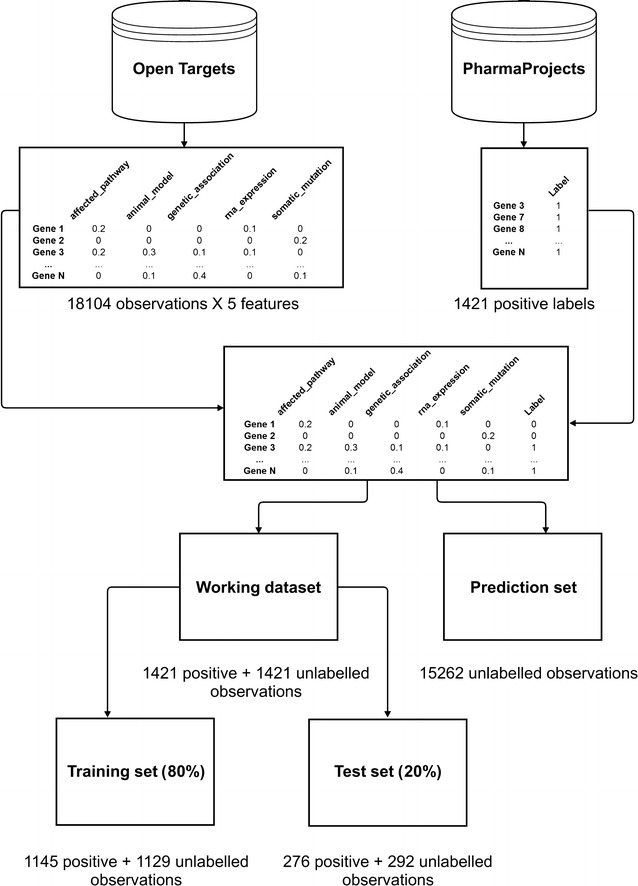
\includegraphics[width=0.5\textwidth]{pics/workflowOpenTargets.jpg}
    \caption{Workflow for the target prediction. While the labels were collected from Informa Pharmaprojects  \cite{pharmaProjects} in the original publication, the results shown here used the targets from Cortellis, provided by Exscientia. The resulting data matrix was split into a \texttt{working set} (1421 positives and 1421 randomly selected unlabelled) and a \texttt{prediction set} (15262 unlabelled genes). The \texttt{working set}, containing both positive and unlabelled observations, was further split into \texttt{training set} and \texttt{test set} to evaluate the performance of the classifier. The \texttt{prediction set} was kept aside and used to perform predictions once all four classifiers was trained}
    \label{fig:ot_workflow}
\end{figure}

Two exploratory analyses were performed: principal component analysis (PCA) (figure \ref{fig:OT_PCA}) and t-Stochastic Neighbourhood Embedding (tSNE) (Figure \ref{fig:OT_tSNE}). Given that the student did not know how these algorithms worked, PCA and the SNE part of t-SNE were coded in Python from scratch (see Annex).

\begin{figure}[H]
\resizebox{\textwidth}{!}{
    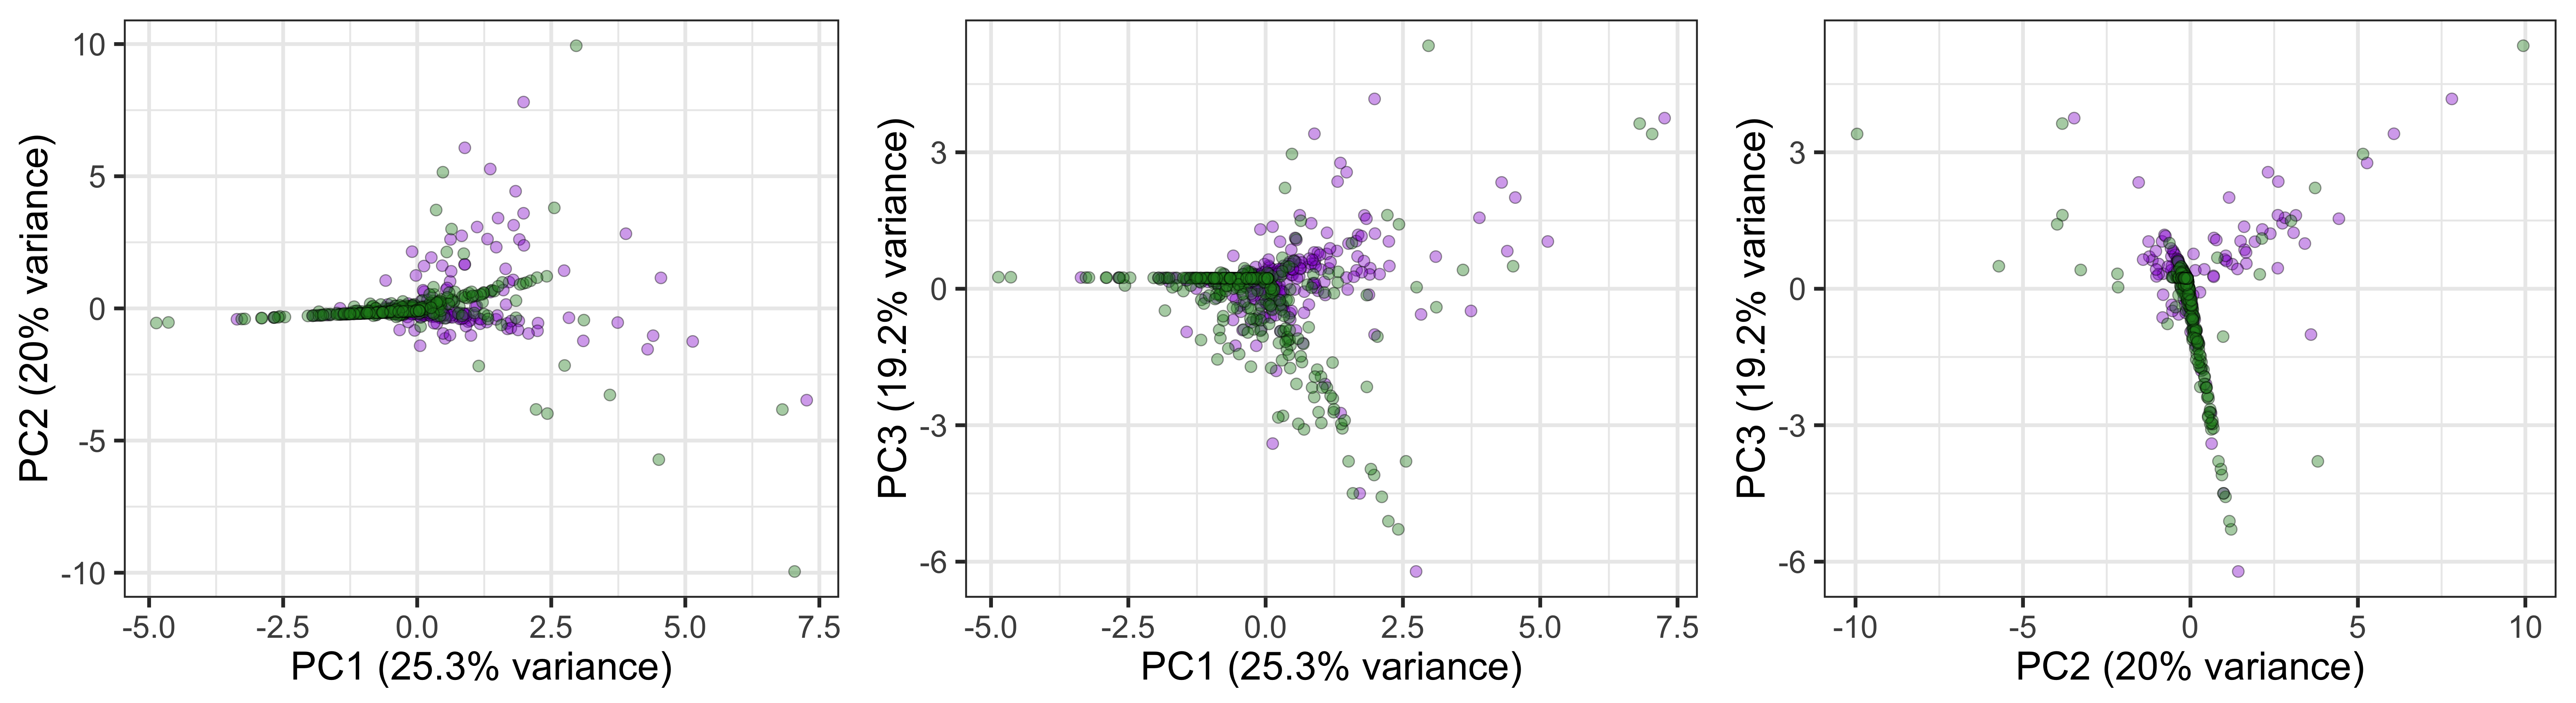
\includegraphics{pics/PCAh.png}}
    \caption{Exploratory data analysis of the \texttt{working set} using PCA for linear dimensionality reduction. Each dot in the two-dimensional space represents a gene and is coloured according to its label (green target, purple non-target)}
    \label{fig:OT_PCA}
\end{figure}

\begin{figure}[H]
\centering
    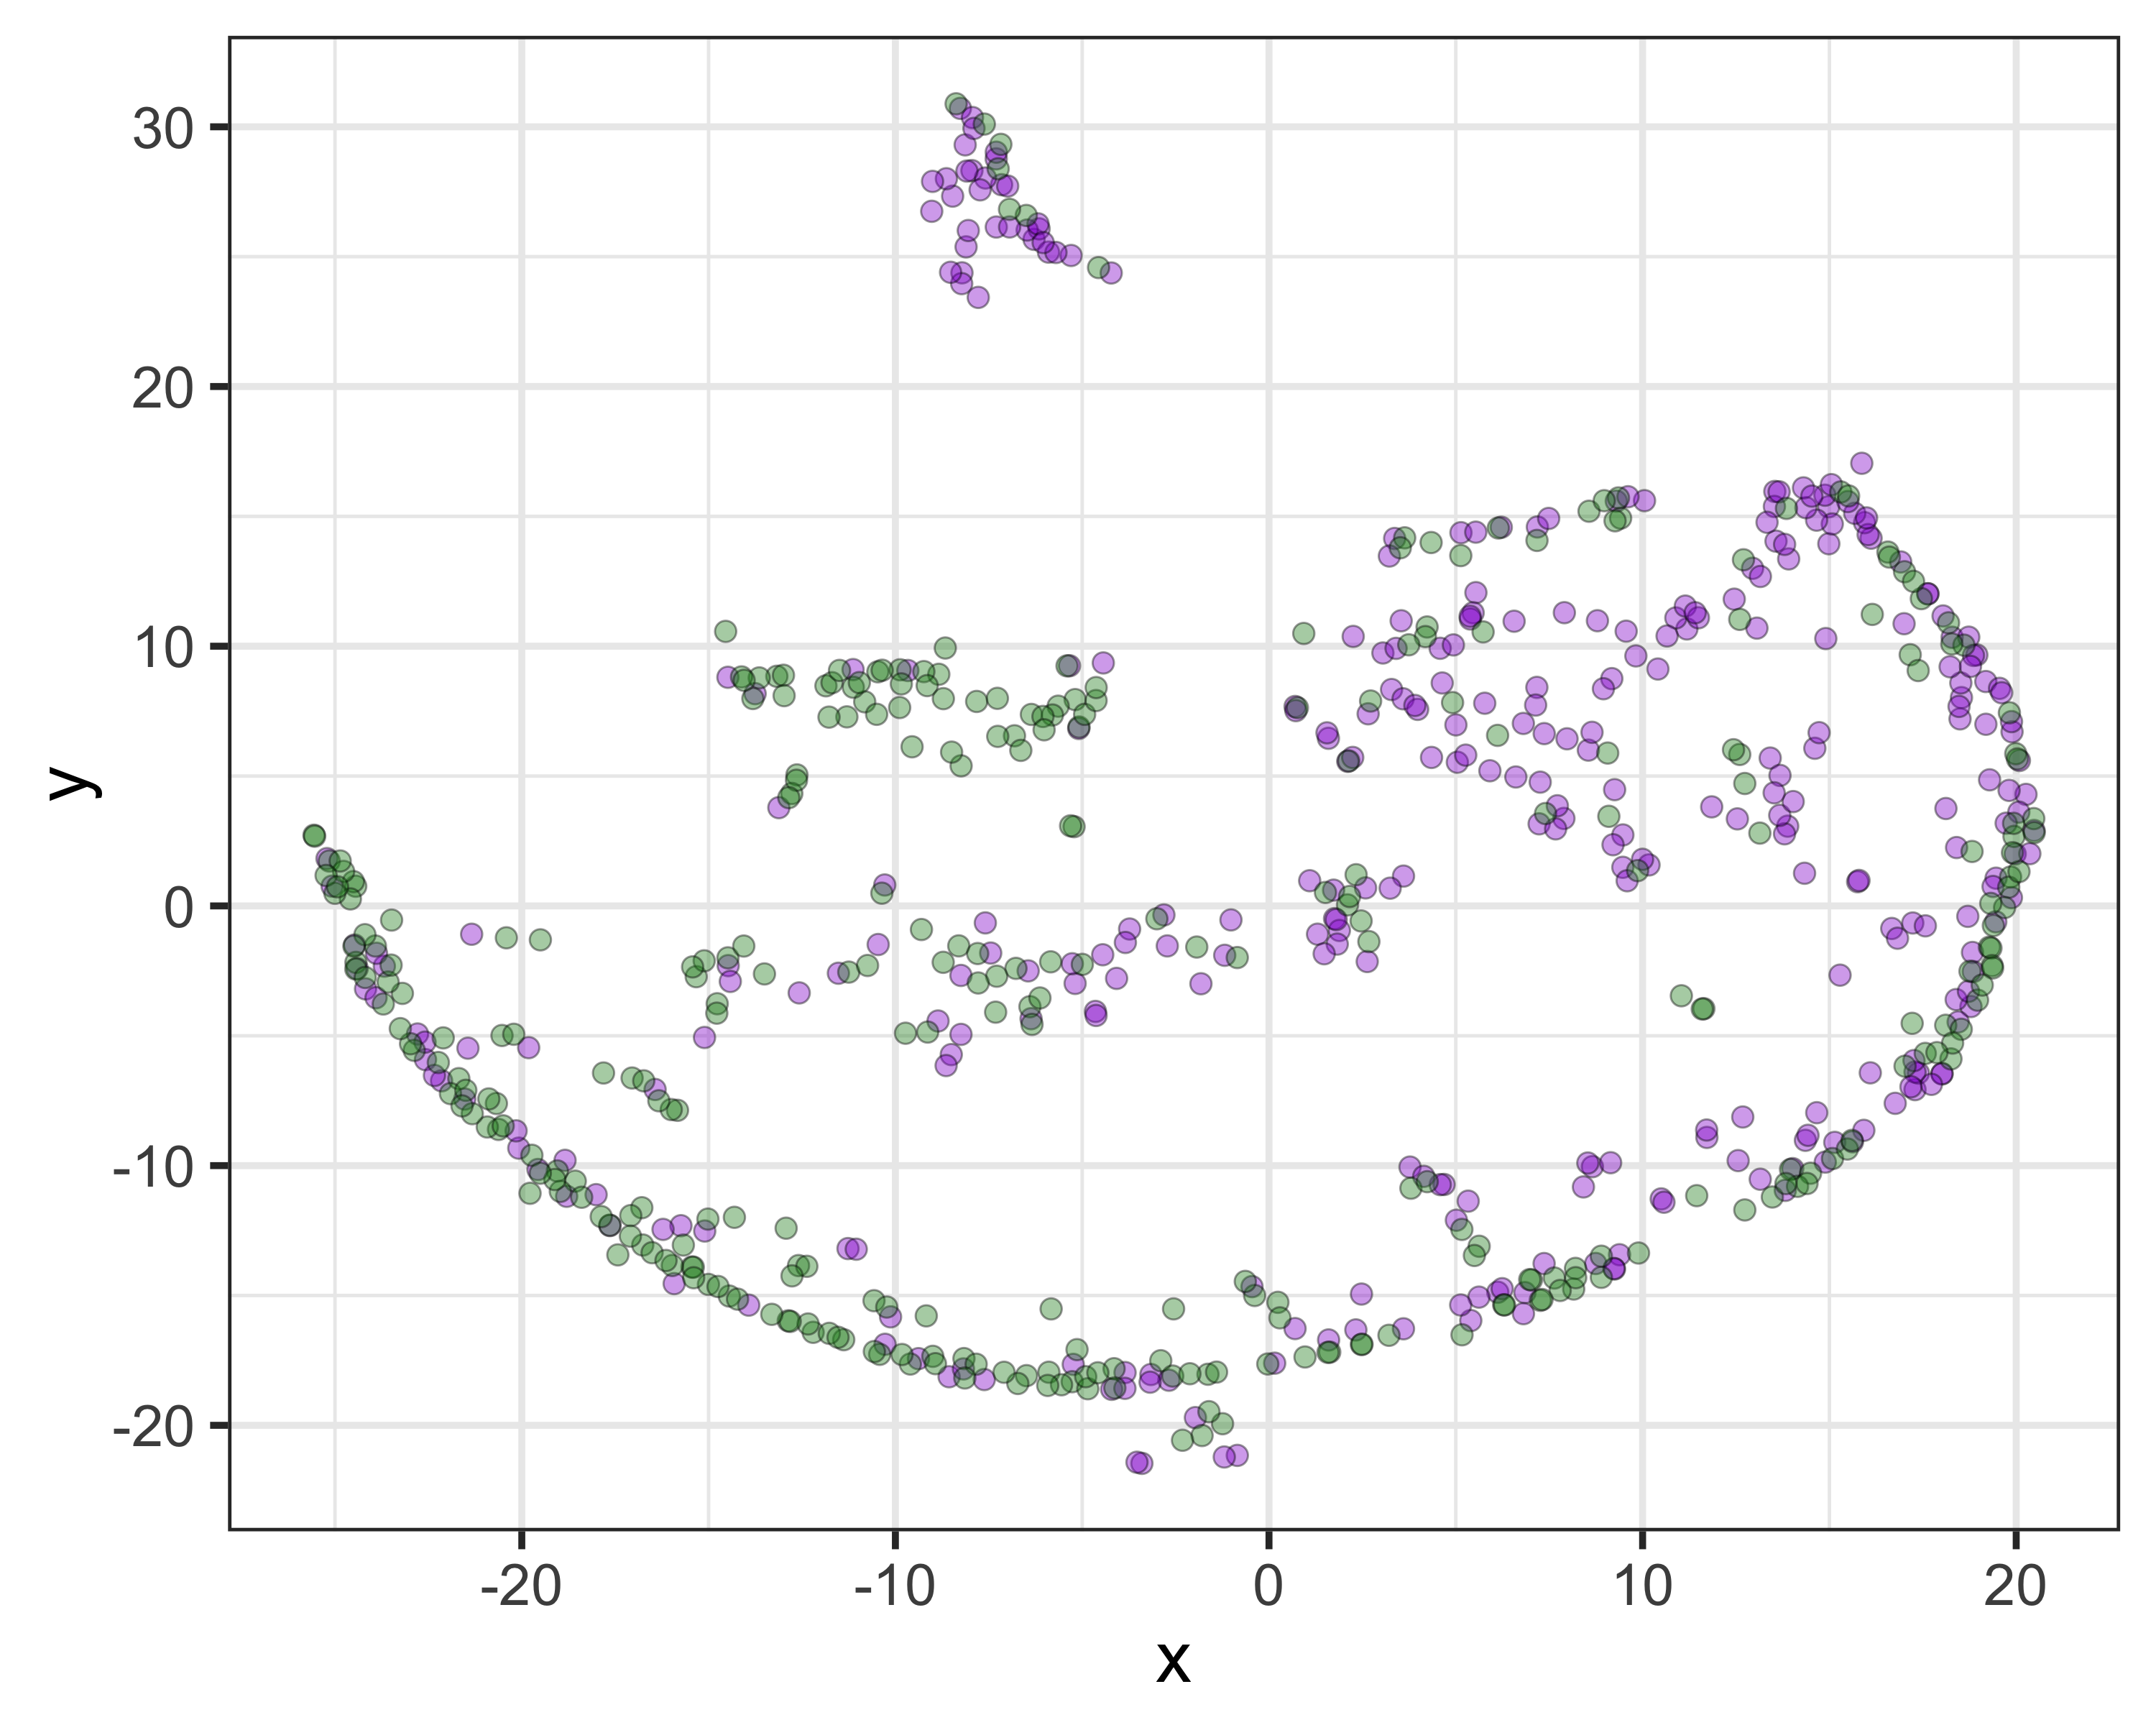
\includegraphics[width=9cm]{pics/tSNE.png}
    \caption{Exploratory data analysis of the \texttt{working set} using dimensionality reduction. The tSNE algorithm for non-linear dimensionality reduction was run a perplexity value of 30 and other default parameters. Each dot in the two-dimensional space represents a gene and is coloured according to its label (green target, purple non-target)}
    \label{fig:OT_tSNE}
\end{figure}

Figure \ref{fig:OT_features} shows the relative importance of each data type whereas Figure \ref{fig:OT_features} represents the classification criteria with a decision tree. In the three approaches, \texttt{animal\_model}, \texttt{rna\_expression} and \texttt{genetic\_association} showed the most informative power. These results are important and will be discussed in Section \ref{subsub:limitations_openTargets}.

\begin{figure}[H]
\subfloat[Feature importance according to Chi Squared test and information gain with the \texttt{working set} \label{fig:OT_features}]{
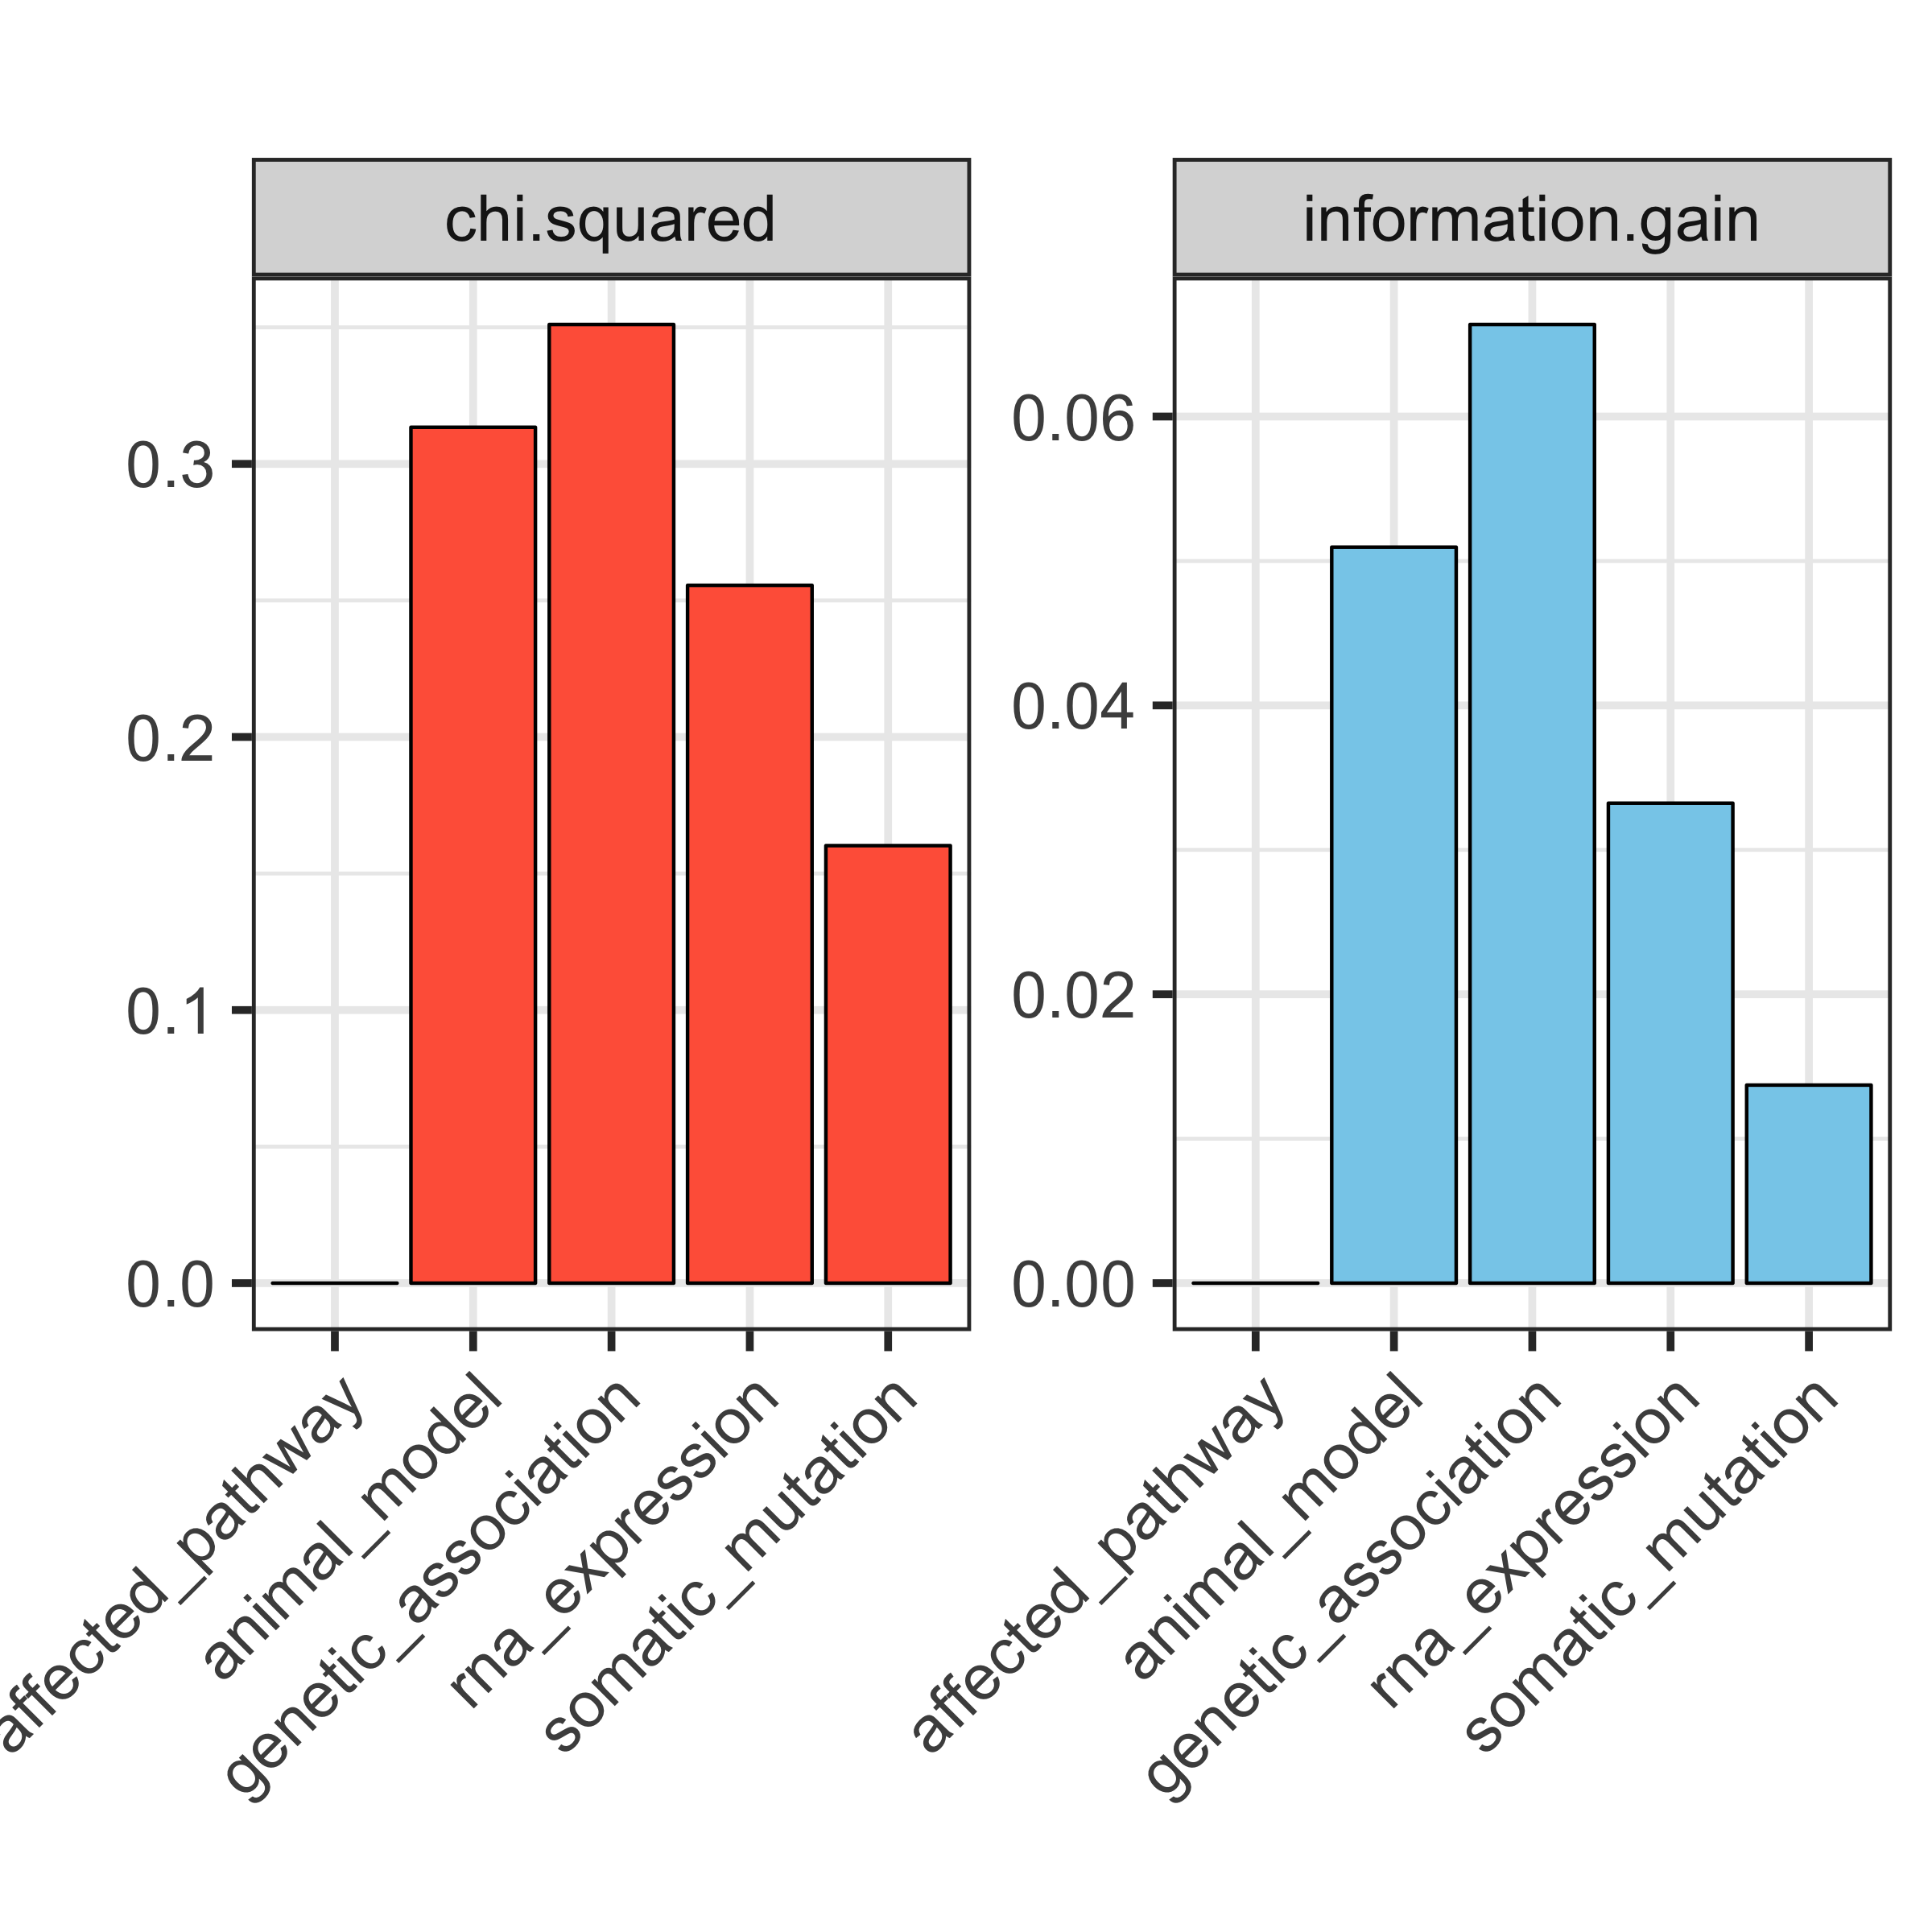
\includegraphics[width=78mm]{pics/Features.png}}
\hfill
\subfloat[Decision tree classification criteria: colours represent predicted outcome (purple: non-target, green: target). In each node, numbers represent (from top to bottom): outcome (FALSE: non-target, TRUE: target), number of observations in node per class (left non-target, right target), percentage of observations in node \label{fig:OT_decisionTree}]{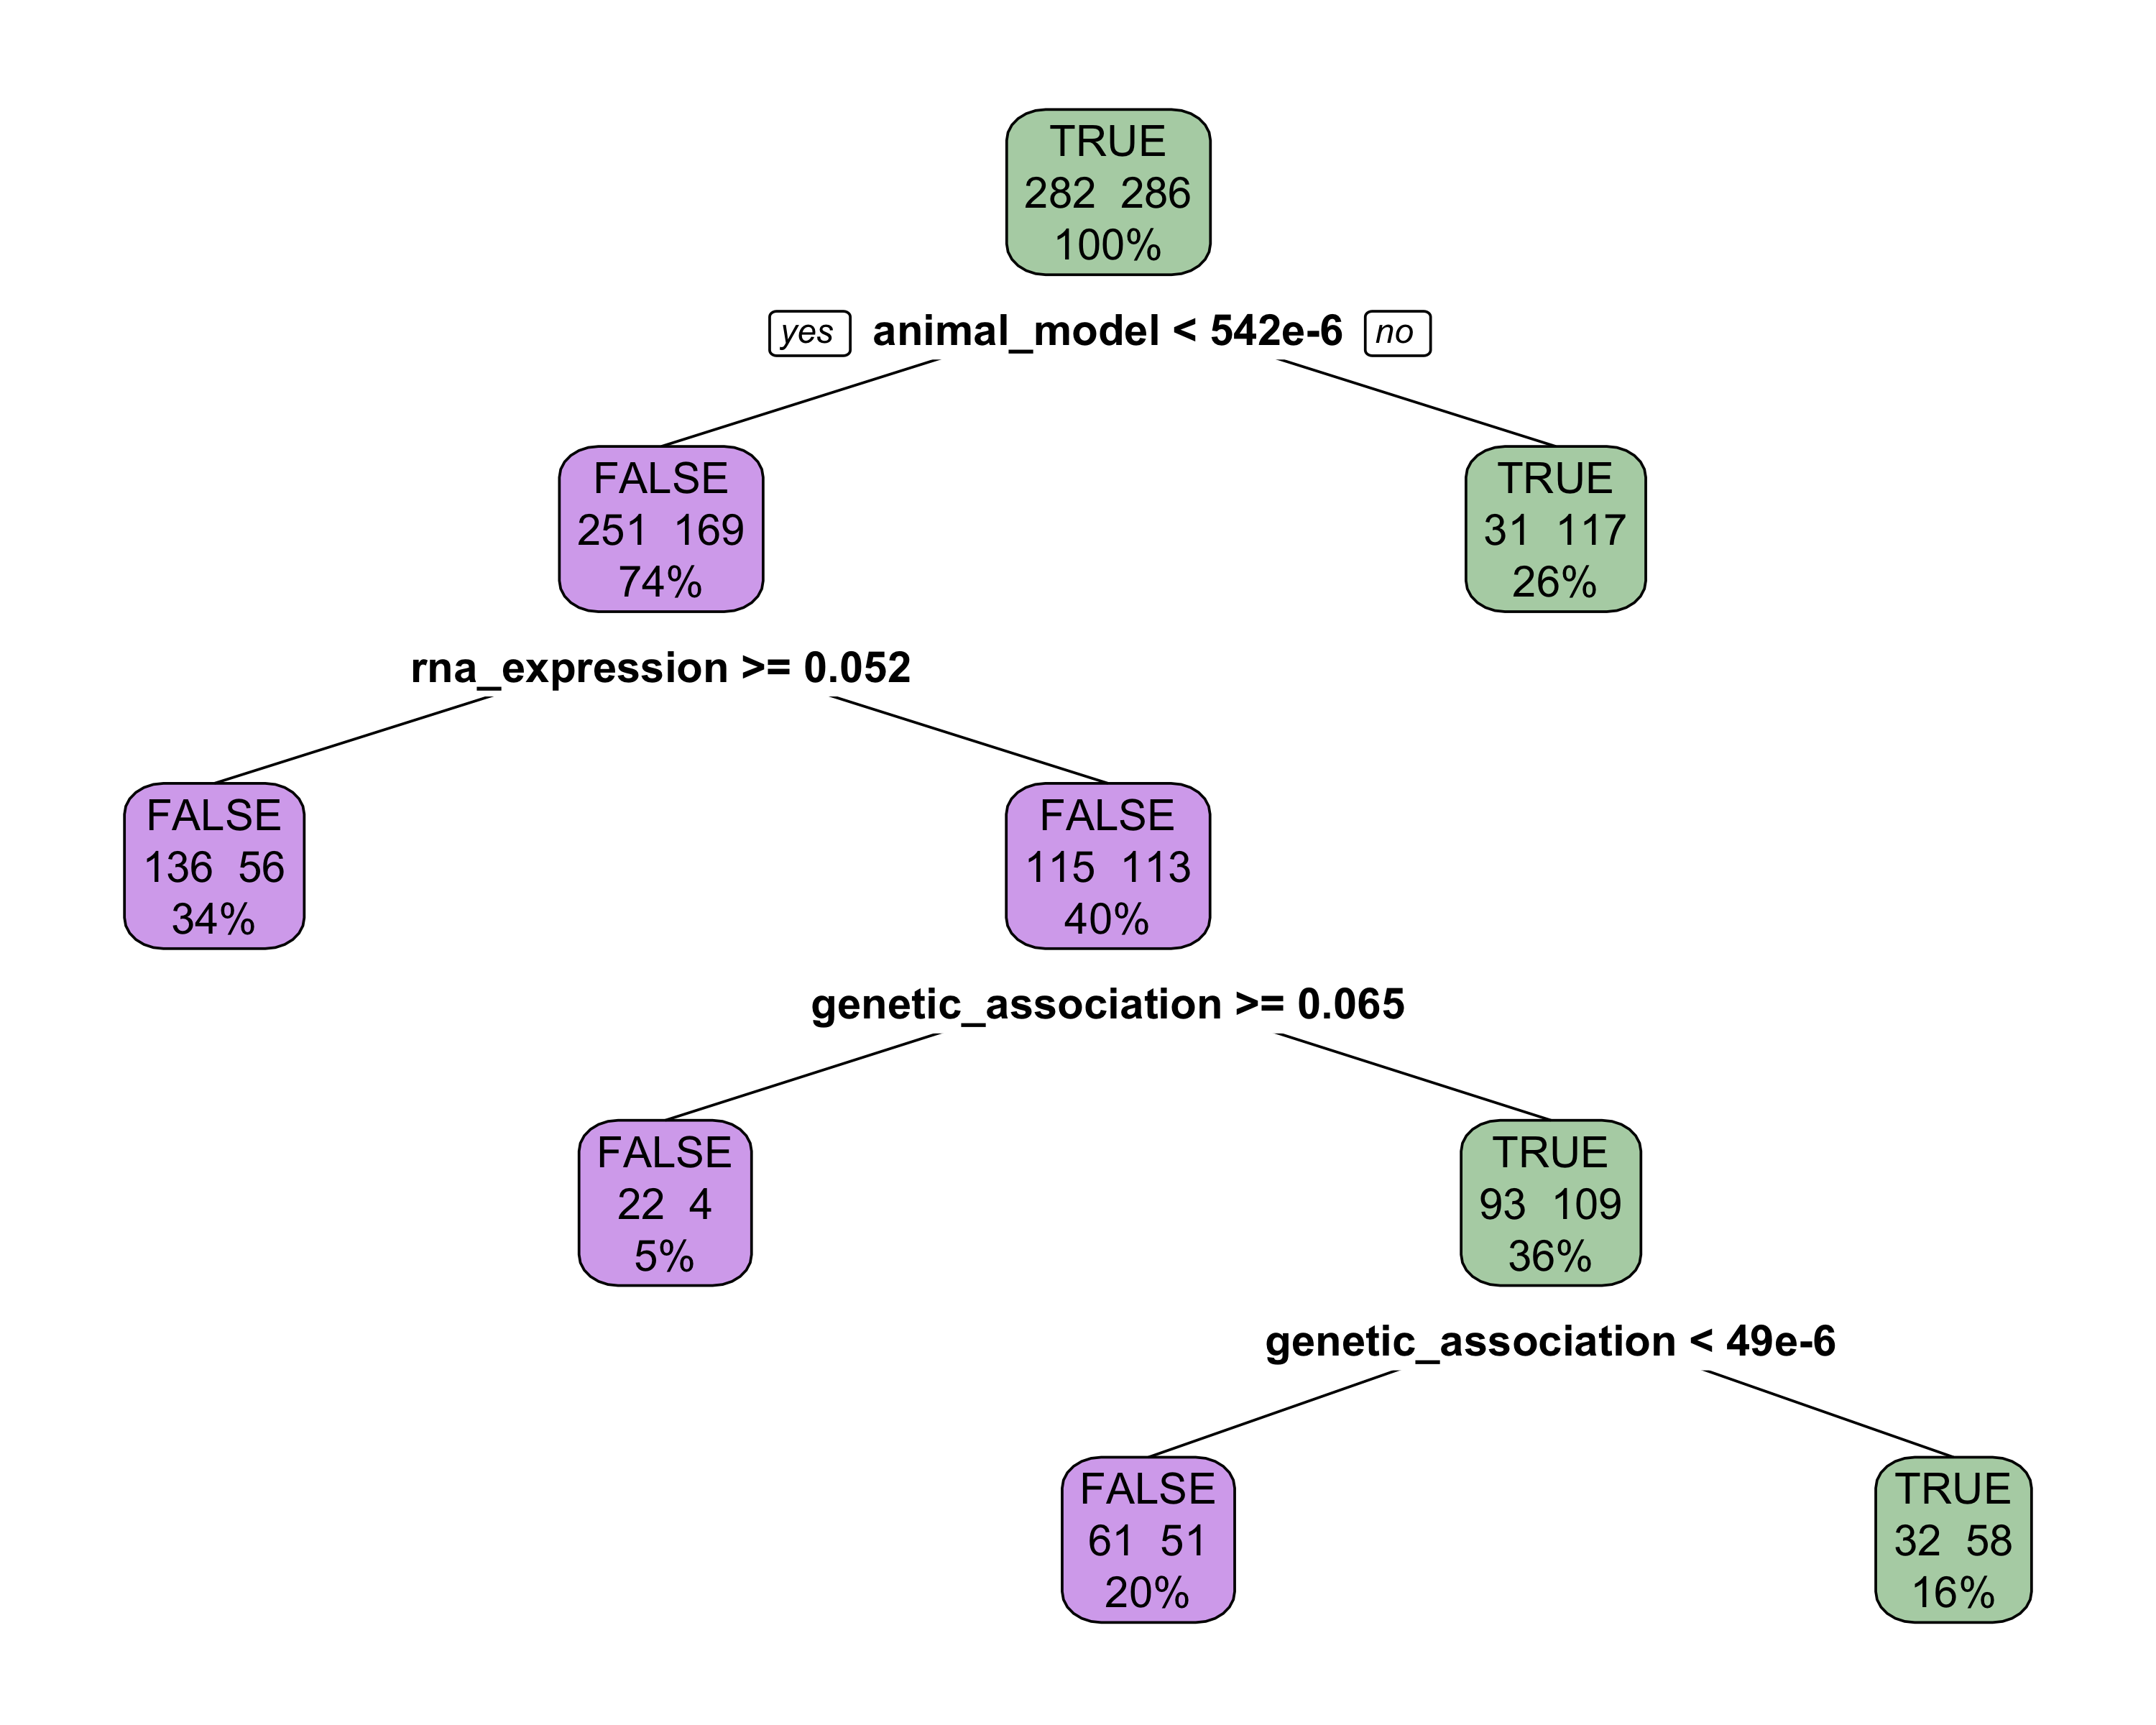
\includegraphics[width=78mm]{pics/DecisionTreeInf.png}}
\end{figure}

Four different classifiers were used, Random Forest (RF), Support Vector Machine (SVM), feed-forward Neural Network (NN) with a single hidden unit, and Gradient Boosting Machine (GBM) in a \emph{semi-supervised} approach on positive unlabelled data with \emph{nested cross-validation} (NCV). Some of the results of the classifiers are displayed in Figure \ref{fig:OT_OtherPlots}. Please refer to \href{https://github.com/davidnarganes/iCASErep}{GitHub repository} for the remaining results.

Why \textbf{semi-supervised}? Data was partially labelled and semi-supervised methods tackle problems when labelling of data is a limitant factor. Just the 8\% of all known human genes were known to be related to drugs. It is uncertain whether the remaining genes may become a potential target in the future \cite{ferrero2017}. 
    
Why \textbf{nested cross-validation} (NCV)? NCV generalises the estimation error of the model and its hyperparameters in an inner loop. Non-NCV biases the model yielding an overly optimistic score. A comparison between NCV and non-NCV in Python can be found \href{https://goo.gl/soHYT7}{elsewhere}.

\begin{figure}[H]
    \centering
    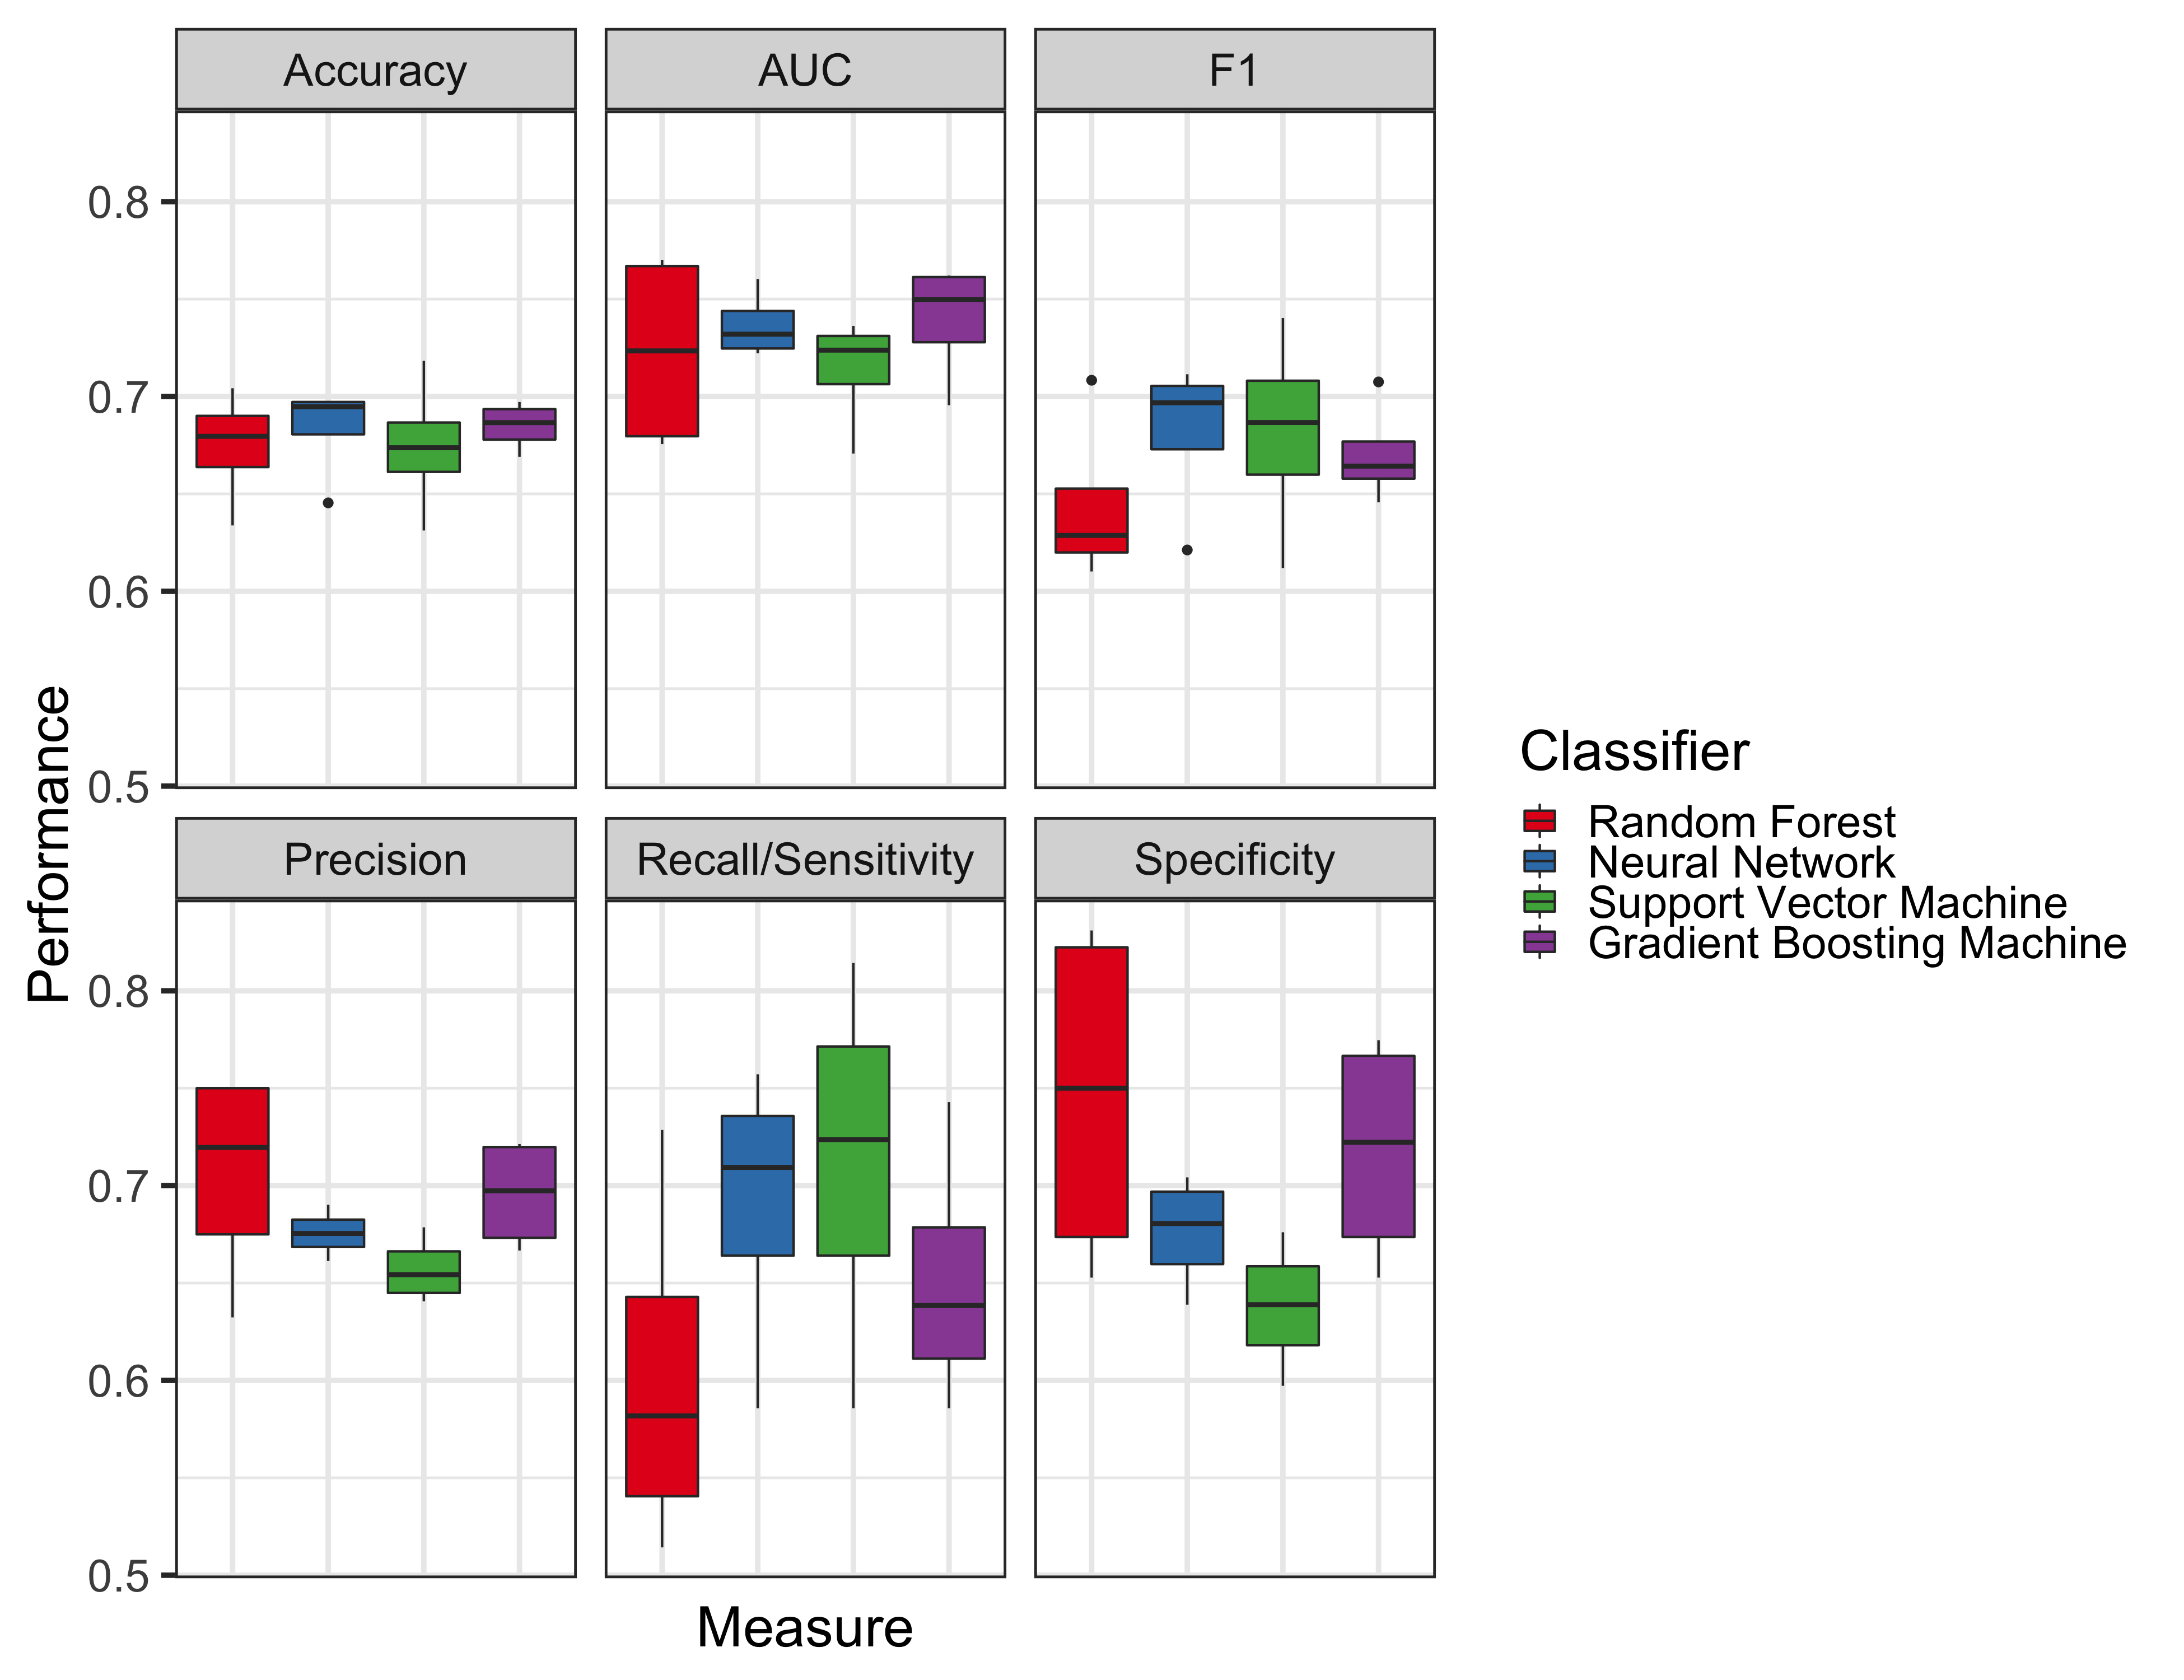
\includegraphics[width = 13cm]{pics/BenchmarkOtherBoxplots.png}
    \caption{Box plots showing distributions of the following measures for the four trained classifiers: accuracy, AUC, F1 measure, precision, recall/sensitivity and specificity, as assessed by NCV on the \texttt{training set} \label{fig:OT_OtherPlots}}
\end{figure}

Overall, all algorithms had comparable accuracy, AUC, and precision (see Figure \ref{fig:OT_OtherPlots}). These results are slightly lower than the ones reported by Ferrero et al. \cite{ferrero2017} (See my results in Table \ref{tab:David_perf_train_mean} and Ferrero's results in Table \ref{tab:OT_perf_train_mean}). 

\begin{table}[H]
\centering
\begin{tabular}{c|c|c|c|c|c|c|c}
Classifier & MMCE  & Accuracy   & AUC   & Recall/Sensitivity   & Specificity   & Precision   & F1    \\
\hline
RF & 0.326 & 0.674 & 0.723 & 0.602 & 0.746 & 0.705 & 0.644 \\
NN & 0.317 & 0.683 & 0.737 & 0.690 & 0.676 & 0.676 & 0.682 \\
SVM & 0.326 & 0.674 & 0.714 & 0.712 & 0.638 & 0.657 & 0.681 \\
GBM & 0.315 & 0.685 & 0.739 & 0.651 & 0.718 & 0.696 & 0.670
\end{tabular}
\caption{\textbf{David results}. Mean \texttt{training set} performance measures (mean misclassification error, mean accuracy, mean AUC, mean recall/sensitivity ratio, mean specificity, mean precision, mean F1 measure) for all classifiers estimated by NCV \label{tab:David_perf_train_mean}}
\end{table}

\begin{table}[H]
\centering
\begin{tabular}{c|c|c|c|c|c|c|c}
Classifier & MMCE  & Accuracy   & AUC   & Recall/Sensitivity   & Specificity   & Precision   & F1    \\
\hline
RF         & 0.302 & 0.698 & 0.761 & 0.596 & 0.802 & 0.753 & 0.665 \\
NN         & 0.303 & 0.697 & 0.758 & 0.610 & 0.785 & 0.742 & 0.670 \\
SVM        & 0.317 & 0.683 & 0.733 & 0.592 & 0.775 & 0.729 & 0.652 \\
GBM        & 0.297 & 0.703 & 0.752 & 0.637 & 0.771 & 0.738 & 0.683
\end{tabular}
\caption{\textbf{Open Targets \cite{ferrero2017}}. Mean \texttt{training set} performance measures (mean misclassification error, mean accuracy, mean AUC, mean recall/sensitivity ratio, mean specificity, mean precision, mean F1 measure) for all classifiers estimated by NCV \label{tab:OT_perf_train_mean}}
\end{table}

The overlap in the classification is reported in Figure \ref{fig:OT_venn}.

\begin{figure}[H]
\resizebox{\textwidth}{!}{
    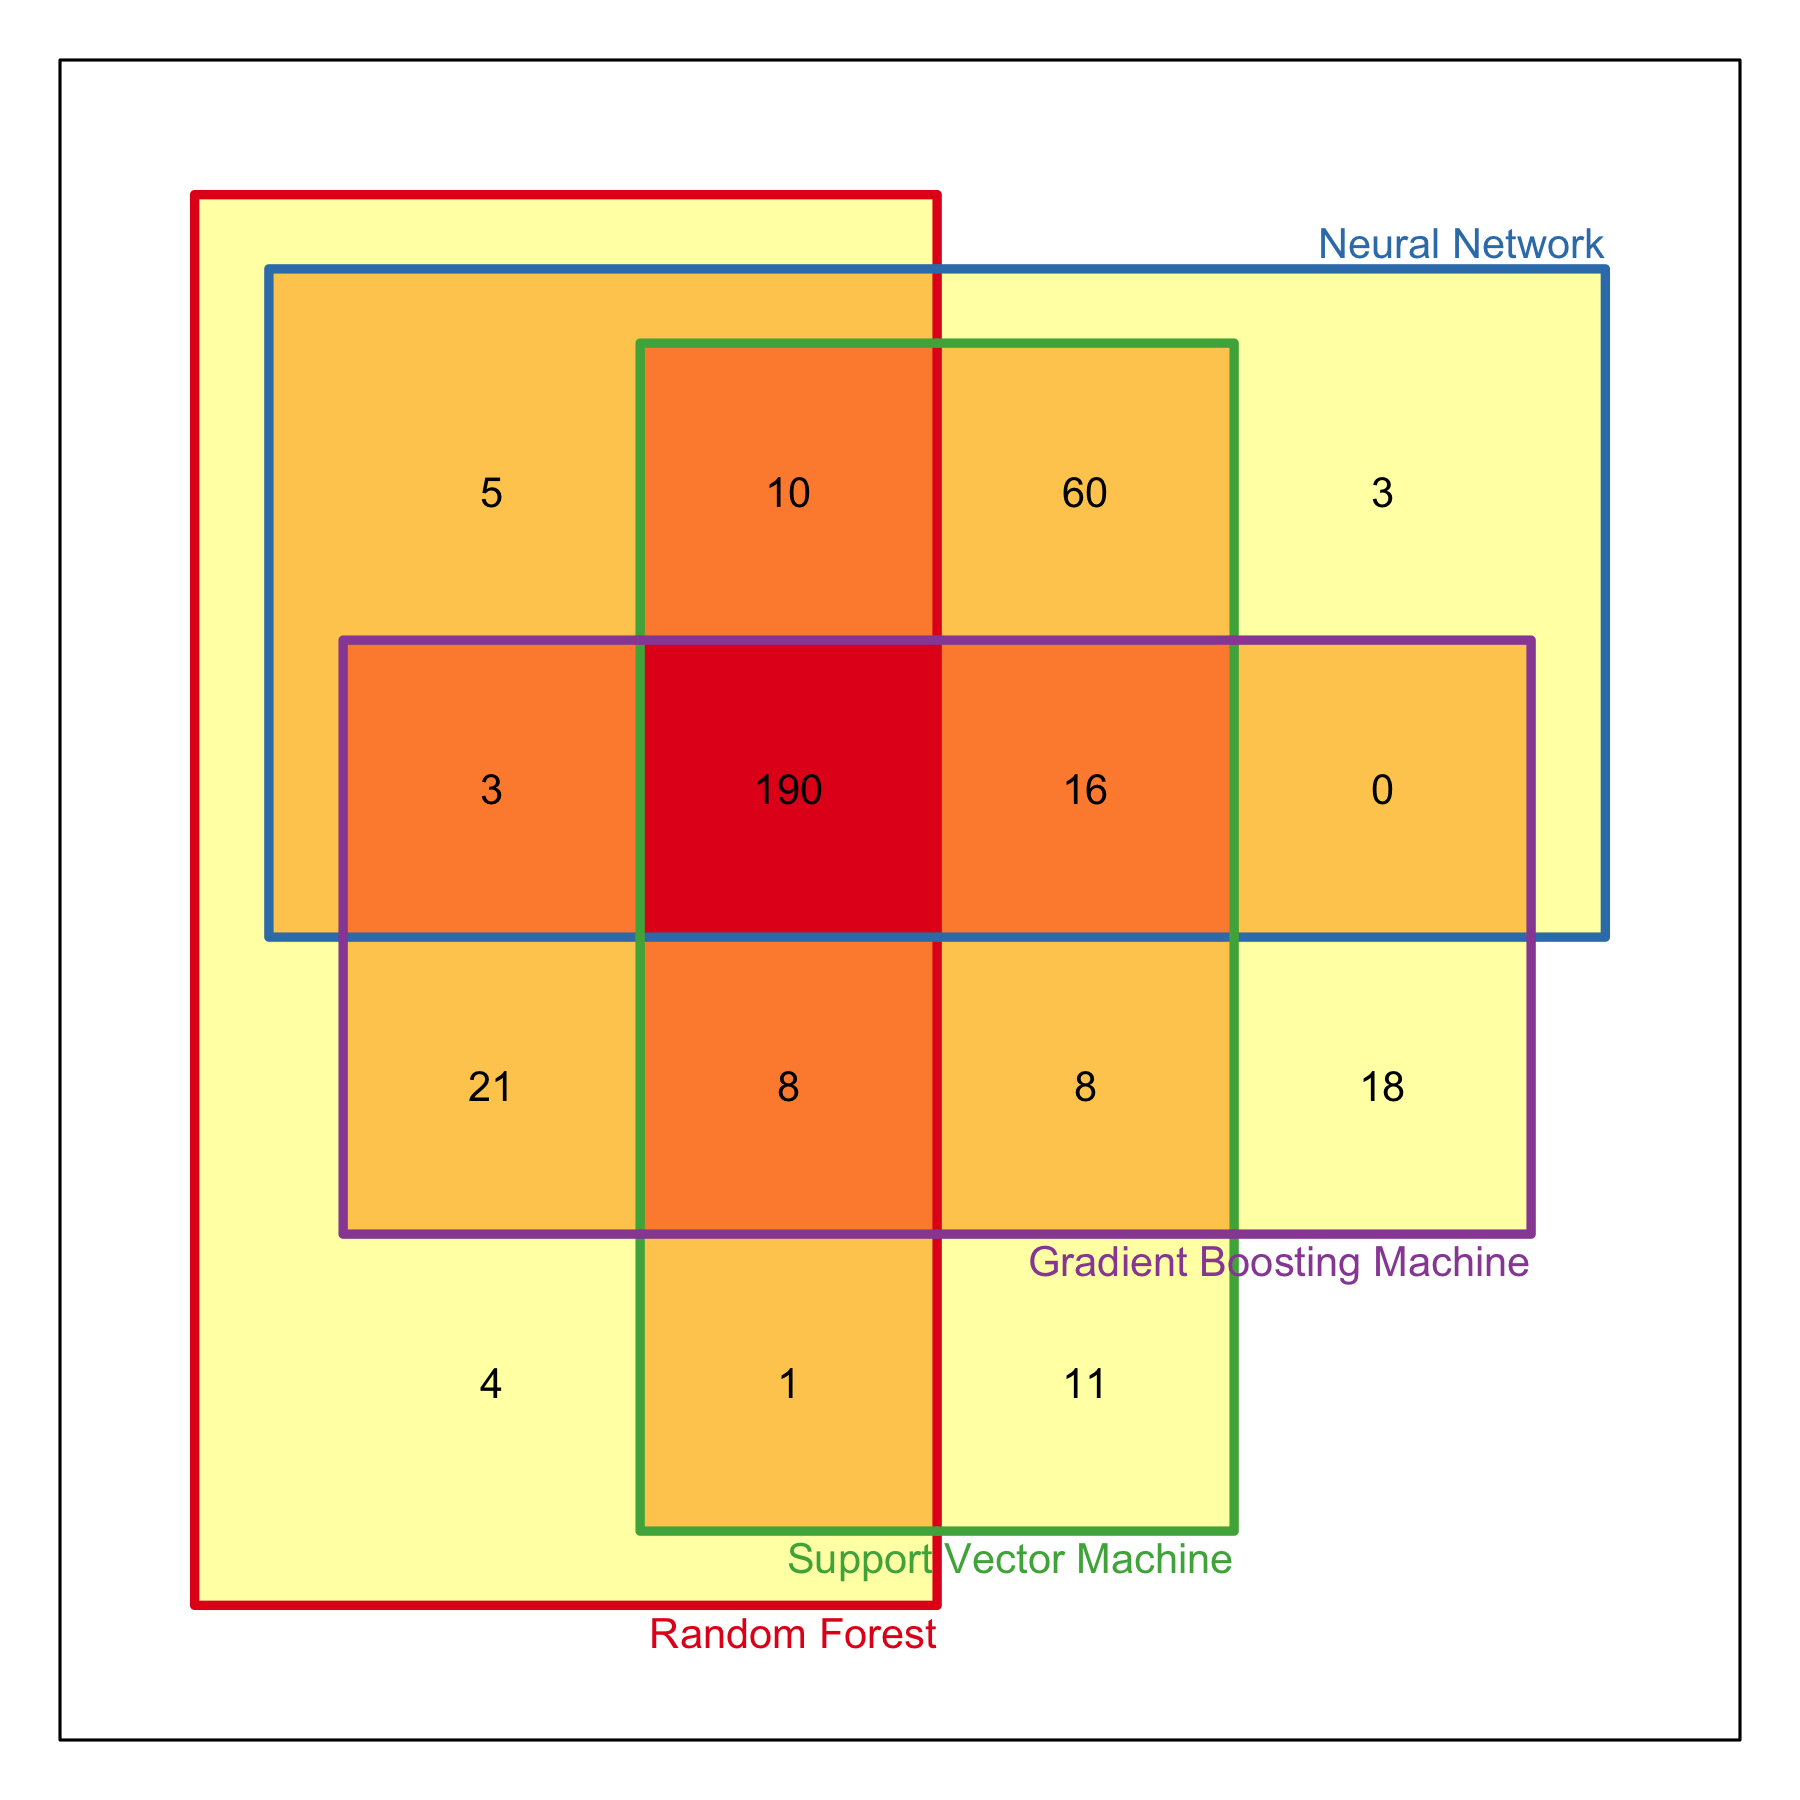
\includegraphics{pics/VennTargets.png}
    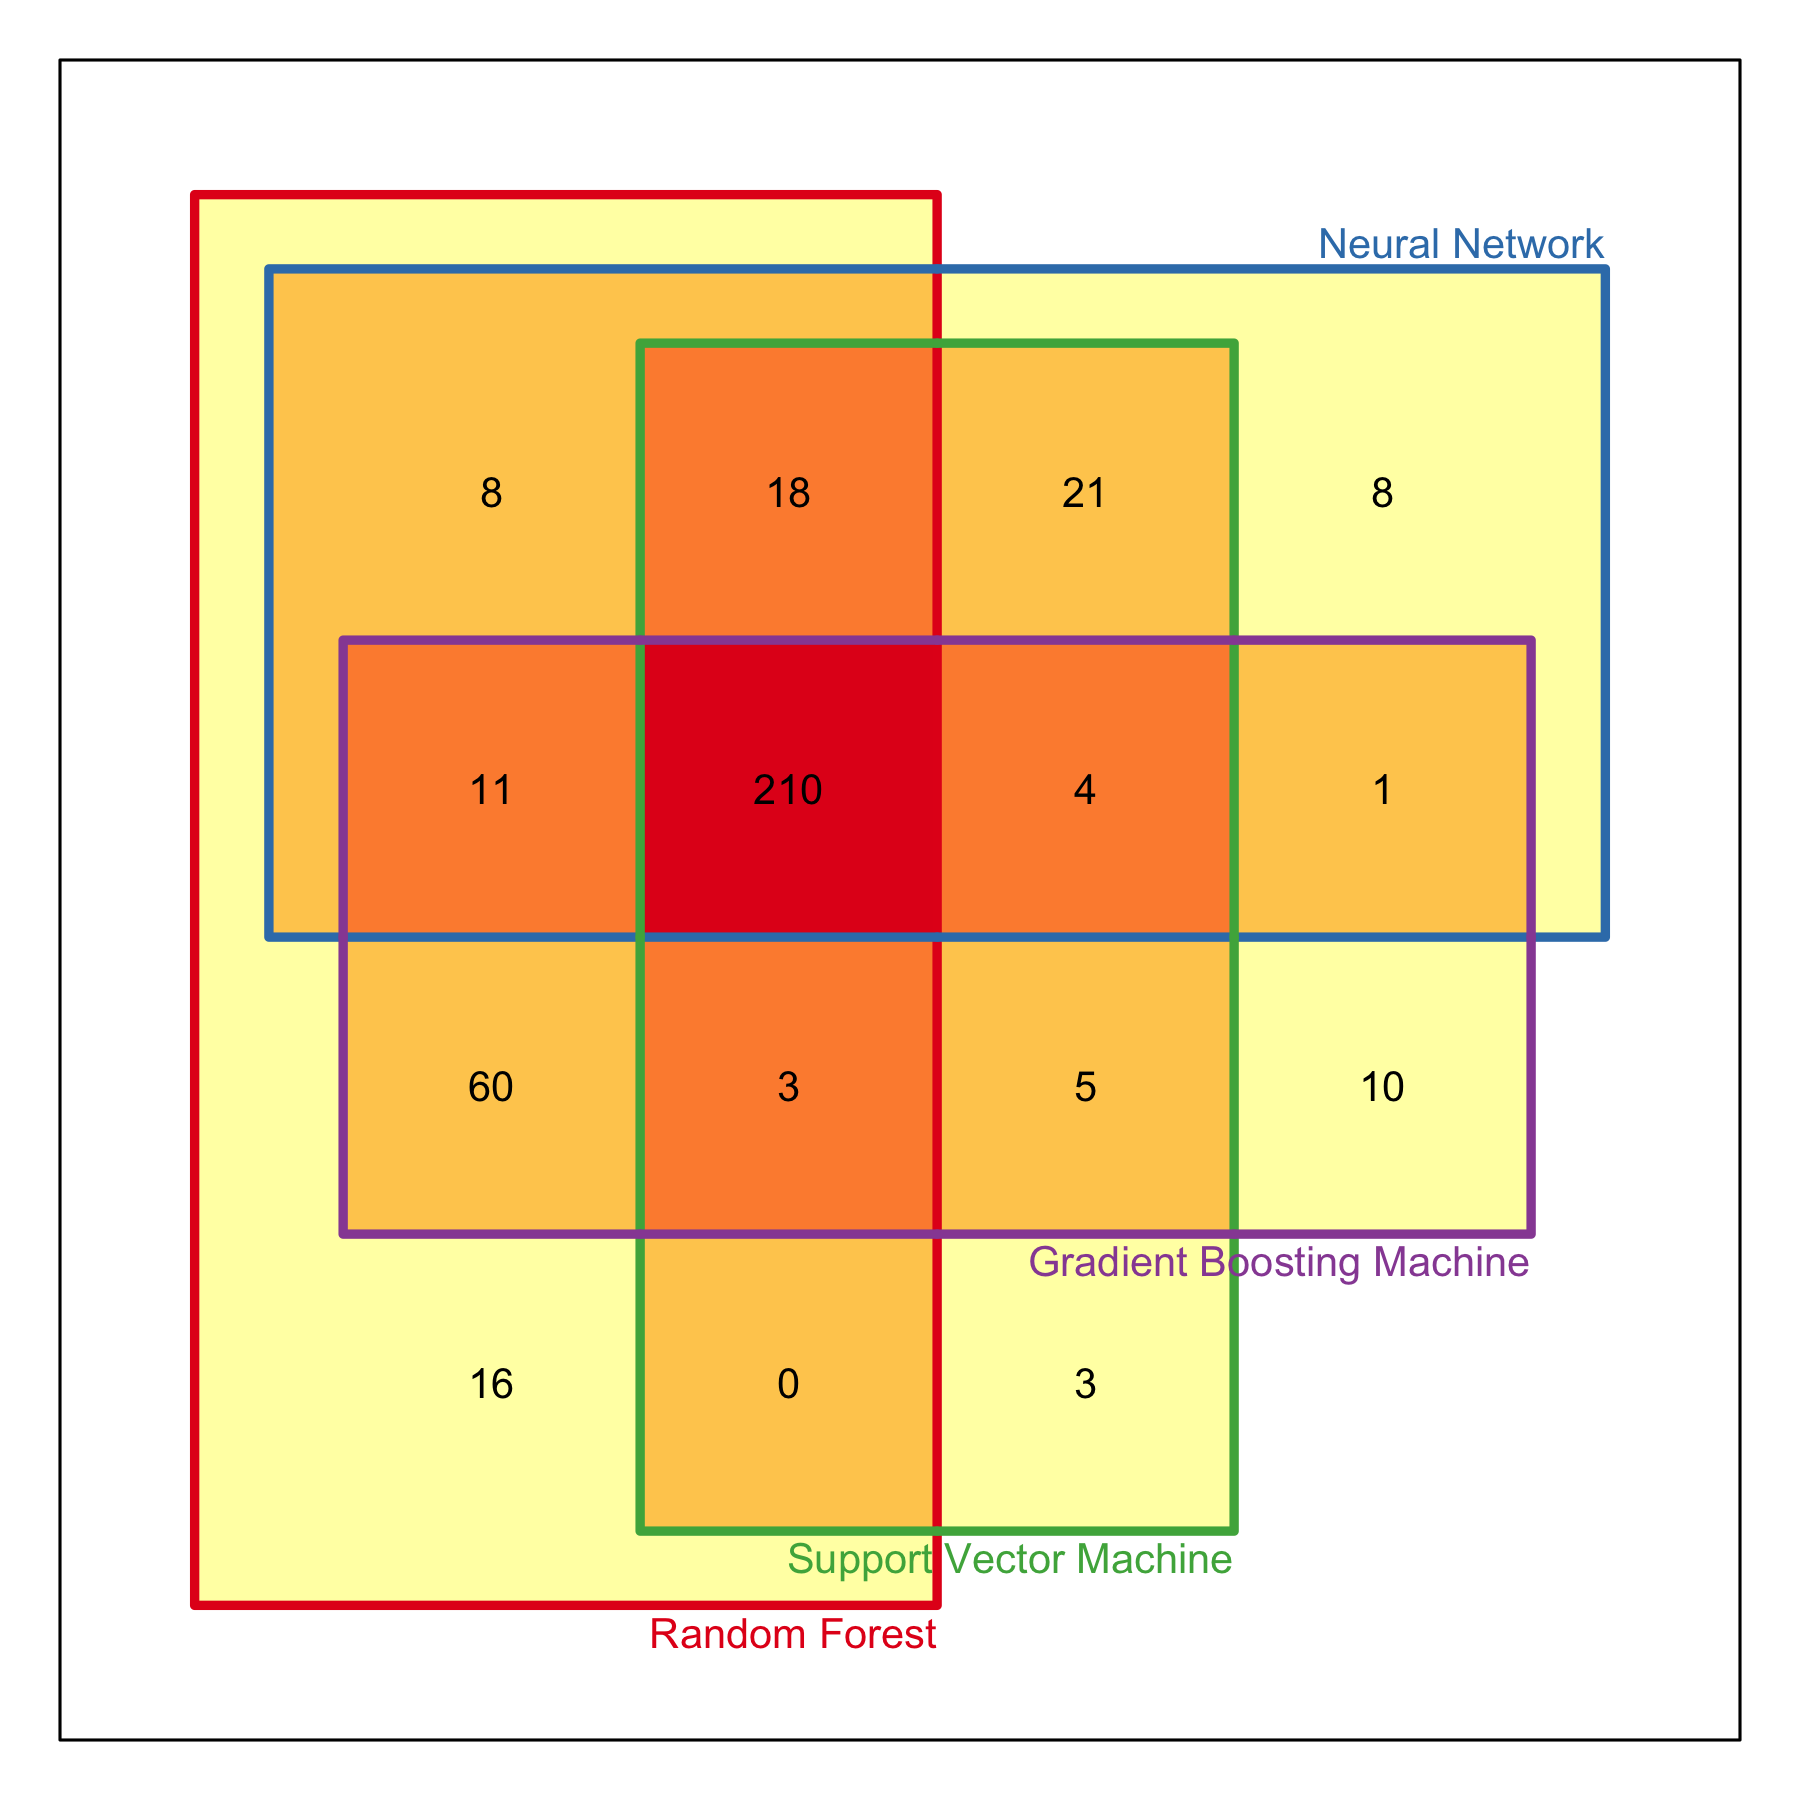
\includegraphics{pics/VennNontargets.png}}
    \caption{Overlap of predicted targets across the four trained classifiers. Venn diagrams showing the relative overlap of predicted targets (left) and predicted non-targets (right) from the \texttt{training set} for the four trained classifiers \label{fig:OT_venn}}
\end{figure}

\subsubsection{Limitations}
\label{subsub:limitations_openTargets}
\begin{enumerate}
    \item \textbf{Labelling of the classes}: there is no pure negative nor positive class which complicates the problem of a binary classification. Nonetheless, defining \emph{bona fide} unsuccessful targets is extremely difficult, if possible at all.
    
    Ferrero et al. \cite{ferrero2017} stated that the unlabelled, negative set contained both future positive targets but from an algorithmic perspective, they simply treated the unlabelled data as the negative set. For this reason, the number of true positives will be  underestimated \cite{ferrero2017}.
    
    Some drugs in early stages of drug development were defined as \emph{positive} successful targets but they may fail in latter stages.
    
    \item The best classifier, the NN, had a poor 71\% accuracy.
    
    \item  Inclusion of functional (Gene Ontology, pathways), structural (protein domains) or interaction data (protein-protein interactions) is likely to have a large impact on the ability to successfully predict targets.
    
    \item Their predictions were individual targets, and not target-disease pairs.
    
    \item Ferrero et al. did not make any claim regarding the druggability of these targets. Open Targets answers questions focused on GDAs but is unable to report focused aspects about the bioactivity profiles of small molecules on those targets \cite{brown2018}
    
    \item Ferrero et al. removed the feature \texttt{literature} since it it was likely to be heavily biased towards well known, validated target–indication pairs. What about \texttt{animal\_model}? Why \texttt{animal\_model} is a good feature for predicting \textbf{novel} therapeutics? The feature \texttt{animal\_model} is a proxy of how much time, research, and money has been spent on a target. Furthermore, their models predicted better later stage targets \cite{ferrero2017}.
    
    \item They claimed that their data types report characteristics that makes good therapeutic targets \cite{ferrero2017} but the main feature is \texttt{animal\_model}. There is no causality, just correlation. The fact of making an experiment about one target on animals does not make that target good. Researchers and companies do not invest money on random targets.
\end{enumerate}

% Disambiguation
\section{Disambiguation of Genes}
\label{section:disambiguation}
The main problem to face was that the literature is filled with alternative, idiosyncratic, and arbitrary gene names and gene symbols from different competing sources that may have other meanings \cite{gad2004,brown2018}. The aim in this section was to develop a novel \href{https://en.wikipedia.org/wiki/Named-entity_recognition}{Name Entity Recogniser} (NER) that uses connected components of papers that are recurrently cocited coupled with machine learning classifiers to locate human gene names in articles from MEDLINE 2018 and 2019. The work done in this section will be continued to (i) allow integration with other relevant databases (see Section \ref{section:lit_review}) and to (ii) develop in the future a novel co-occurrence gene-disease ranking coupled with semantic analysis to account for the positivity or negativity of the GDAs.

\subsection{Workflow}
The workflow of the NER is detailed in Figure \ref{fig:NER_workflow}.
\begin{figure}
    \centering
    \includegraphics{}
    \caption{Caption}
    \label{fig:NER_workflow}
\end{figure}

 - gene or disease may have other meanings
 - contextual information from nearby words
 - comprehensive dictionary of genes is a prerequisite for text mining
 - gene associations extracted from Medline abstracts
 - disguise human from orthologs based on synonyms
 
PROBLEMS:
- papers in cluster cocited not talking about gene
- all clusters with safe synonyms -> No training data, all positive class
- No safe synonyms -> all negative class
- 

% Bibliography
\bibliographystyle{plain}
\bibliography{refs}

% % Appendix
% \appendix
% \section{Principal Component Analysis}
% \subsection{Introduction}

Often, the desired goal is to reduce the dimensions of a N-dimensional dataset by projecting it onto a k-dimensional subspace (where k\textless N) in order to increase the computational efficiency while retaining most of the information.

A summary of the Principal Component Analysis is the following:
\begin{enumerate}
    \item Standarise the data
    \item Obtain the covariance matrix
    \item Obtain the \emph{eigenvectors} and their correspondent \emph{eigenvalues}
    \item Sort the eigenvalues in descending order of magnitude to chose the \emph{k} eigenvectors that correspond to the \emph{k} largest eigenvalues
    \item Construct the projection matrix \emph{\textbf{W}} from the selected \emph{k} eigenvectors
    \item Transform the original dataset \emph{\textbf{X}} via \emph{\textbf{W}} to obtain a k-dimensional feature subspace \emph{\textbf{Y}}
\end{enumerate}

\subsection{Standarisation}
All variables must be on the same scale with a \texttt{standard scaler}:

$$
x_d = \frac{x_d - \overline{x}_d}{\sqrt{
\sum \frac{(x_d - \overline{x}_d)^2}{N}}}
$$

Here is the code:
\begin{lstlisting}[language=Python]
import numpy as np

# 0. Define data
X = np.random.rand(200,10)

# Make X not to be in scale 0-1
d = np.random.poisson(20,10)
X = np.multiply(X,d)

def standarisation(X):
    for d in range(X.shape[1]):
        X[:,d] = (X[:,d] - X[:,d].mean()) / X[:,d].std()
    return X

# 1. Standarise data
X_std = standarisation(X.copy())
\end{lstlisting}

\subsection{Covariance matrix, Eigenvalues, and Eigenvectors}
The classic approach to PCA is to perform the eigendecomposition on the covariance matrix $\Sigma$, which is a $d \cdot d$ matrix where each element represents the covariance between two variables, calculated as follows:

$$
\sigma_{j,k} = \frac{1}{n-1}\sum_{i=1}^N {(x_{i,j} - \overline{x}_{j})} \cdot {(x_{i,k} - \overline{x}_{k})}
$$

With some algebra, this equation can be summarised into:
$$
\Sigma = \frac{1}{n-1}\sum_{i=1}^N {(X - \overline{x})^T}{(X - \overline{x})}
$$

In Python code:

\begin{lstlisting}[language=Python]
# Get mean
mean_vec = np.mean(X_std, axis=0)

# 2. Get covariance matrix
cov_mat = (X_std - mean_vec).T.dot((X_std - mean_vec)) / (X_std.shape[0]-1)
\end{lstlisting}

Next, eigenvalues and the eigenvectors are obtained:

\begin{lstlisting}[language=Python]
# 3. Eigen decomposition
eig_vals, eig_vecs = np.linalg.eig(cov_mat)
\end{lstlisting}

Sometimes, they are calculated with the correlation matrix \textbf{\emph{X}}. Nevertheless, this method yields the same results since the correlation matrix can be understood as the normalized covariance matrix. This statement is tested here:

\begin{lstlisting}[language=Python]
# 3. Eigendecomposition
cov_mat = np.cov(X_std.T)
eig_vals, eig_vecs = np.linalg.eig(cov_mat)
print(eig_vals)

[Out]:[ 1.43557072  0.62102126  0.77387224  0.79279969  1.20947608  1.15829268
  0.93869466  0.99929095  1.07098582  1.05024716]

# 4. Test cor_mat
cor_mat1 = np.corrcoef(X_std.T)
eig_vals_, eig_vecs_ = np.linalg.eig(cor_mat1)
print(eig_vals_)

[Out]: [ 1.42839287  0.61791616  0.77000288  0.78883569  1.2034287   1.15250122
  0.93400118  0.99429449  1.06563089  1.04499592]

\end{lstlisting}

\subsection{Sort eigenvalues}
Which eigenvector(s) can dropped without losing too much information? Eigenvectors with the lowest eigenvalues bear the least information about the distribution of the data and, therefore, they can be dropped.

The eigenvalues are ranked to choose the top \emph{k} eigenvectors:

\begin{lstlisting}[language=Python]
# 5. Sort eigenvalues
eig_pairs = [(np.abs(eig_vals[i]), eig_vecs[:,i]) for i in range(len(eig_vals))]
eig_pairs.sort()
eig_pairs.reverse()
\end{lstlisting}

\subsection{Explained variance}

How many principal componets we choose for the new feature space? A useful measure is the \emph{explained variance}. The explained variance is calculated from the eigenvalues and tells us how much information or variance can be attributed to each of the principal components. It can be calculated and plotted as follows:

\begin{lstlisting}[language=Python]
import matplotlib.pyplot as plt
import datetime
import os
fig, ax1 = plt.subplots()
components = range(len(var_exp))
color = 'deeppink'
ax1.set_xlabel('Components')
ax1.set_ylabel('Explained Variance', color=color)
ax1.bar(components, var_exp, color=color)
ax1.tick_params(axis='y', labelcolor=color)

ax2 = ax1.twinx()  # instantiate a second axes that shares the same x-axis
color = 'blue'
ax2.set_ylabel('Cumulative Explained Variance', color=color)
ax2.errorbar(components, cum_var_exp, marker='o', color=color, ls='dotted')
ax2.tick_params(axis='y', labelcolor=color)
plt.xlabel('Components')
plt.xticks(list(components))
fig.tight_layout()
dirpath = '/Users/dnarganes/PhD/PCA_raw/pics'
if not os.path.exists(dirpath):
    os.makedirs(dirpath)
filename = 'img_{}.png'.format(datetime.datetime.now())
plt.savefig(os.path.join(dirpath,filename))
\end{lstlisting}

\begin{figure}[H]
\centering
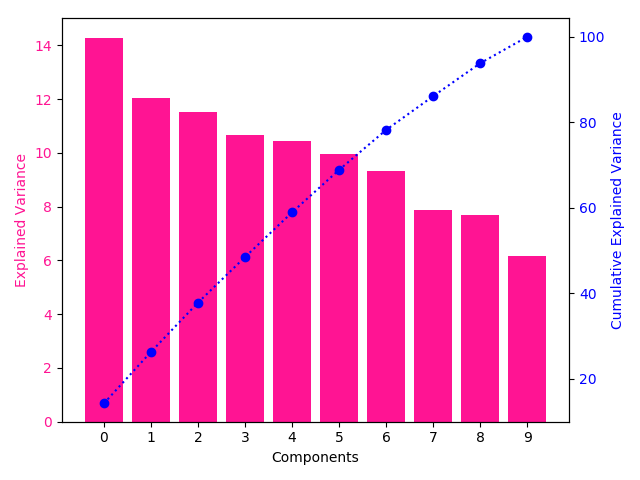
\includegraphics[width=12cm]{pics/pca_var_exp.png}
\end{figure}

The above plot shows that the first three components account for the 0.3 of the variance. Take into account that the defined matrix \emph{\textbf{X}} was defined as from a normal random distribution. With a real dataset I could take the first \emph{k} components that account for most of the variance.

\subsection{Y and W matrices}
The aim is to reduce the \emph{d} dimensional feature space to a 2 dimensional feature subspace by choosing the top 2 eigenvectors to make the reduced eigenvector matrix \emph{\textbf{W}}. Finally, the dot product of \emph{\textbf{X}} and \emph{\textbf{W}} matrices gives me the \emph{\textbf{Y}} matrix.

\begin{lstlisting}[language=Python]
# 6. Projection onto new feature subspace
matrix_w = np.hstack((eig_pairs[0][1].reshape(len(components),1), 
                      eig_pairs[1][1].reshape(len(components),1)))

Y = X_std.dot(matrix_w)
print(Y.shape)

[Out]: (200,2)
\end{lstlisting}



% \section{Stochastic Neighbourhood Embedding}
% \subsection{Introduction}
This is an attempt to understand of some of the most frequently-used machine learning methods by using just base Python and numpy.

t-Stochastic Neighbourhood Embedding is a dimensionality reduction algorithm. This means we can take some data that lives in a high-dimensional space (such as images, which usually consist of thousands of pixels), and visualise it in a lower-dimensional space. This is desirable, as humans are much better at understanding data when it is presented in a two- or three-dimensional space.

\subsection{SNE}
t-distributed Stochastic Neighbour Embedding, or t-SNE, was developed by Geoffrey Hinton and Laurens van der Maaten in \hyperlink{http://www.jmlr.org/papers/volume9/vandermaaten08a/vandermaaten08a.pdf}{this paper}. This appendix will just cover the SNE part.

\subsubsection{P matrix}

Given a dataset $X$ with $N$ data points and $D$ dimensions, the aim is to reduce it to $d$ dimensions: e.g. $d=2$ without losing generality. SNE converts the euclidean distance between data points to conditional probabilities of likelihood to be a neighbour.

$$ P_{j|i}=\frac{exp(-||x_i - x_j||^2 / 2\sigma^2_i)}{\sum_{k\neq i}^kexp(-||x_i - x_k||^2 / 2\sigma^2_i)} $$

This is, the probability of point $x_j$ to be a neighbour of point $x_i$ is proportional to de distance between this two points. $\sigma$ will be explained later as well as the denominator.

\emph{Note}: $p_{i|i}=0$ for all $i$ since it is irrelevant how much of a neighbour each point is with itself.

\subsubsection{Q matrix}
The $Q$ matrix is a $N\times2$ dimensional matrix, the output of t-SNE and the 2D representation of $X$.

$$ Q_{j|i}=\frac{exp(-||x_i - x_j||^2)}{\sum_{k\neq i}^kexp(-||x_i - x_k||^2)} $$

\subsubsection{KL divergence}
The overall goal is to get points $q_i$ such that the conditional probability distribution $q_i$ is similar to $p_i$. This is achieved by minimising a cost function: the \hyperlink{https://en.wikipedia.org/wiki/Kullback-Leibler_divergence}{Kullback–Leibler divergence} or KLD between these two distributions. KLD or $C$ is defined as follows:

$$ C = \sum_i KLD(P_i||Q_i) = \sum_i \sum_j P_{j,i} \log(\frac{P_{j|i}}{Q_{j|i}}) $$

The function will be minimised with \hyperlink{https://en.wikipedia.org/wiki/Gradient_descent}{gradient descent}. This will be explained later. To calculate the negative squared distances:
\begin{lstlisting}[language=Python]
def neg_squared_euc_dists(X):
    sum_X = np.sum(np.square(X), 1)
    D = np.add(np.add(-2 * np.dot(X, X.T), sum_X).T, sum_X)
    return -D
\end{lstlisting}

It returns an $N\times N$ matrix that contain the euclidean distances for all $x_i$ and $x_j$.

Also, I will need the softmax function for the denominator of the formulas for matrices $P$ and $Q$:
\begin{lstlisting}[language=Python]
def softmax(X, diag_zero=True):

    # Subtract max to scale
    e_x = np.exp(X - np.max(X, axis=1).reshape(-1, 1))

    # We usually want diagonal probabilities to be 0
    if diag_zero:
        np.fill_diagonal(e_x, 0.)

    # Add a tiny constant to avoid log problems
    e_x = e_x + 1e-16

    return e_x / e_x.sum(axis=1).reshape(-1, 1)
\end{lstlisting}

To get the matrix $P$:
\begin{lstlisting}[language=Python]
def get_P(distances, sigmas=None):
    """Convert a distances matrix to a matrix of probabilities."""
    if sigmas is not None:
        two_sig_sq = 2. * np.square(sigmas.reshape((-1, 1)))
        return softmax(distances / two_sig_sq)
    else:
        return softmax(distances)
\end{lstlisting}

\subsubsection{Perplexity}
In the previous code snippet, the sigmas argument should be an N-length vector containing each of the $\sigma_i$. This is achieved with the \hyperlink{https://en.wikipedia.org/wiki/Perplexity}{perplexity}. The perplexity of any of the rows $P_i$ of the conditional probabilities matrix $P$ is defined as:
$$ Perp(P_i) = 2^{H(P_i)}$$

Where $H(P_i)$ is the \href{https://en.wiktionary.org/wiki/Shannon_entropy}{Shannon entropy} of $P_i$ in bits:
$$ H(P_i) = - \sum p_{j|i} \log_2 (p_{j|i}) $$

In SNE, perplexity usually has a value between 5 and 50\footnote{\url{https://scikit-learn.org/stable/modules/generated/sklearn.manifold.TSNE.html}}. We then set each $\sigma_i$ such that for each row of $P$, the perplexity of that row is equal to our desired perplexity, the parameter we set.

\emph{Note}: Probability distributions with high entropy (and therefore high perplexity) are relatively flat: elements have similar probabilities. In SNE, high perplexity makes the $P_{j|i}$ similar to each other, the probability of being a neighbour is similar for all reasonably close points. The larger the perplexity, the larger the $\sigma_i$ we divide by, the closer the probability distribution gets to having all probabilities equal to just 1/N. This is why perplexity is set to the number of neighbours we believe each point has\footnote{\url{https://scikit-learn.org/stable/modules/generated/sklearn.manifold.TSNE.html}}.

To ensure the perplexity of each row of $P$, $Perp(Pi)$, is equal to the desired perplexity, it is required a binary search over each $\sigma_i$ until $Perp(Pi)$ is close enough to the desired perplexity. This is possible because $Perp(Pi)$ is a \hyperlink{https://en.wikipedia.org/wiki/Monotonic_function}{monotonically increasing function} of $\sigma_i$.

The binary search function is:
\begin{lstlisting}[language=Python]
def binary_search(eval_fn, target, tol=1e-10, max_iter=10000, lower=1e-20, upper=1000.):
    for i in range(max_iter):
        guess = (lower + upper) / 2.
        val = eval_fn(guess)
        if val > target:
            upper = guess
        else:
            lower = guess
        if np.abs(val - target) <= tol:
            break
    return guess
\end{lstlisting}

To find the $\sigma_i$ it is necessary to pass an \emph{eval\_fn} to \emph{binary\_search} function that takes a given $\sigma_i$ as its argument and returns the perplexity of $P_i$ with that $\sigma_i$.


The \emph{find\_optimal\_sigmas} function below does exactly this to find all $\sigma_i$. It takes a matrix of negative euclidean distances and a target perplexity. For each row of the distances matrix, it performs a binary search over possible values of $\sigma_i$ until finding that which results in the target perplexity. It then returns a \texttt{numpy} vector containing the optimal $\sigma_i$.

\begin{lstlisting}[language=Python]
def calc_perplexity(prob_matrix):
    entropy = -np.sum(prob_matrix * np.log2(prob_matrix), 1)
    perplexity = 2 ** entropy
    return perplexity

def perplexity(distances, sigmas):
    return calc_perplexity(calc_prob_matrix(distances, sigmas))

def find_optimal_sigmas(distances, target_perplexity):
    sigmas = [] 
    # For each row of the matrix (each point in our dataset)
    for i in range(distances.shape[0]):
        # Make fn that returns perplexity of this row given sigma
        eval_fn = lambda sigma: \
            perplexity(distances[i:i+1, :], np.array(sigma))
        # Binary search over sigmas to achieve target perplexity
        correct_sigma = binary_search(eval_fn, target_perplexity)
        # Append the resulting sigma to our output array
        sigmas.append(correct_sigma)
    return np.array(sigmas)
\end{lstlisting}

\subsubsection{Symmetric SNE}

Now, it is possible to find a 2D representation $Y$ by descending the gradient of the cost $C$ with respect to $Y$ until convergence. The gradient of SNE is more complicated to implement so in this report it will be used the Symmetric SNE. Symmetric SNE was described as 'just as good' alternative to tSNE.

\textbf{Difference}: Symmetric SNE minimises a KL divergence over the \emph{joint} probability distributions with entries $p_{i,j}$ and $q_{i,j}$, as opposed to conditional probabilities $p_{i|j}$ and $q_{i|j}$. With the joint distribution, each $q_{i,j}$ is given by:

$$ Q_{j|i}=\frac{exp(-||x_i - x_j||^2)}{\sum_{k\neq l}^kexp(-||x_k - x_l||^2)} $$

This is just like the softmax in the denominator we had before, except now the normalising term in the denominator is summed over the entire matrix $l$, rather than just the current row $i$.

To avoid problems related to outlier $X$ points:
$$ p_{ij}= \frac{p_{i|j} + p_{j|i}}{2N}$$

The code:
\begin{lstlisting}[language=Python]
def q_joint(Y):
    # Get the distances from every point to every other
    distances = neg_squared_euc_dists(Y)
    # Take the elementwise exponent
    exp_distances = np.exp(distances)
    # Fill diagonal with zeroes so q_ii = 0
    np.fill_diagonal(exp_distances, 0.)
    # Divide by the sum of the entire exponentiated matrix
    return exp_distances / np.sum(exp_distances), None


def p_conditional_to_joint(P):
    return (P + P.T) / (2. * P.shape[0])
    
def p_joint(X, target_perplexity):
    # Get the negative euclidian distances matrix for our data
    distances = neg_squared_euc_dists(X)
    # Find optimal sigma for each row of this distances matrix
    sigmas = find_optimal_sigmas(distances, target_perplexity)
    # Calculate the probabilities based on these optimal sigmas
    p_conditional = calc_prob_matrix(distances, sigmas)
    # Go from conditional to joint probabilities matrix
    P = p_conditional_to_joint(p_conditional)
    return P
\end{lstlisting}

\subsubsection{Gradient descent SNE}
After differencing the KLD, gradient descent is used to update the i'th row of our low dimensional representation $Y$:
$$ G = \frac{\partial C}{\partial y_i} = 4\sum_j (p_{ij} - q_{ij}) (y_i - y_j)$$

\begin{lstlisting}[language=Python]
def symmetric_sne_grad(P, Q, Y, _):
    pq_diff = P - Q  # NxN matrix
    pq_expanded = np.expand_dims(pq_diff, 2)  #NxNx1
    y_diffs = np.expand_dims(Y, 1) - np.expand_dims(Y, 0)  #NxNx2
    grad = 4. * (pq_expanded * y_diffs).sum(1)  #Nx2
    return grad
\end{lstlisting}

In this function, G is an $N\times2$ matrix whose i’th row is $\partial C / \partial y_i$

Afterwards, update the $y_i$ row of the $Y$ matrix:
$$Y^t_i = Y_i^{t-1} - \mu \frac{\partial C}{\partial y_i}$$

The update of the gradient descent has to be done iteratively:

\begin{lstlisting}[language=Python]
def estimate_sne(X, y, P, rng, num_iters, q_fn, grad_fn, learning_rate, momentum, plot):

    # Initialise our 2D representation
    Y = rng.normal(0., 0.0001, [X.shape[0], 2])

    # Initialise past values (used for momentum)
    if momentum:
        Y_m2 = Y.copy()
        Y_m1 = Y.copy()

    # Start gradient descent loop
    for i in range(num_iters):

        # Get Q and distances (distances only used for t-SNE)
        Q, distances = q_fn(Y)
        # Estimate gradients with respect to Y
        grads = grad_fn(P, Q, Y, distances)

        # Update Y
        Y = Y - learning_rate * grads
        if momentum:  # Add momentum
            Y += momentum * (Y_m1 - Y_m2)
            # Update previous Y's for momentum
            Y_m2 = Y_m1.copy()
            Y_m1 = Y.copy()

        # Plot sometimes
        if plot and i % (num_iters / plot) == 0:
            categorical_scatter_2d(Y,
            y,
            alpha=1.0,
            ms=6,
            show=True,
            figsize=(9, 6))

    return Y
\end{lstlisting}

\newpage
\subsubsection{Results: MNIST dataset}

\begin{figure}[H]
\centering
\subfloat[0 iterations]{
  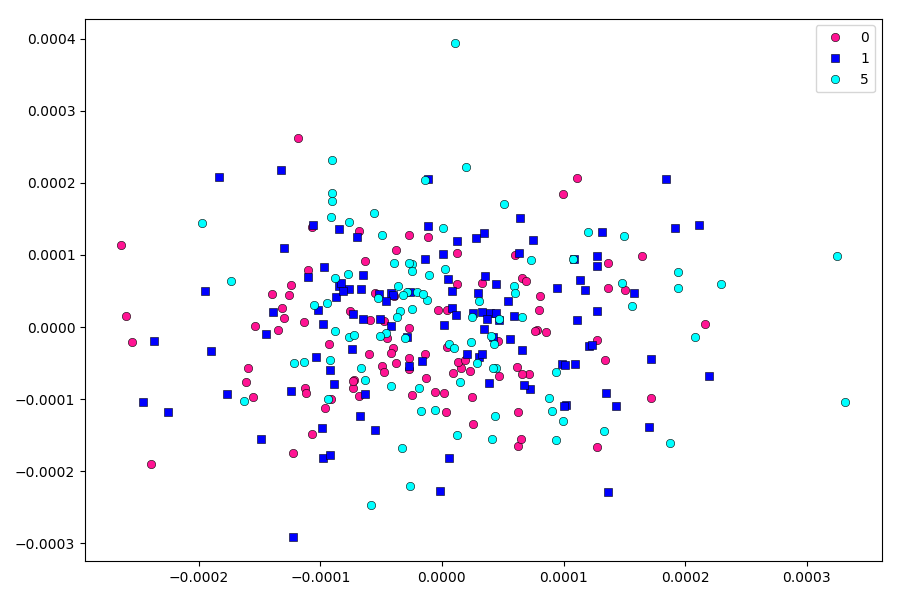
\includegraphics[width=53mm]{pics/tsne_False_iter_0.png}
}
\subfloat[10 iterations]{
  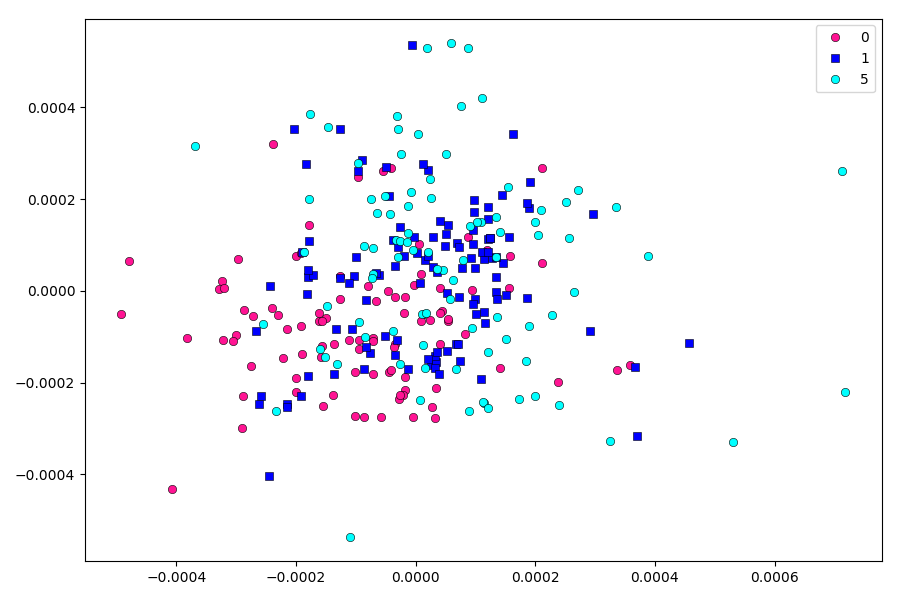
\includegraphics[width=53mm]{pics/tsne_False_iter_10.png}
}
\subfloat[20 iterations]{
  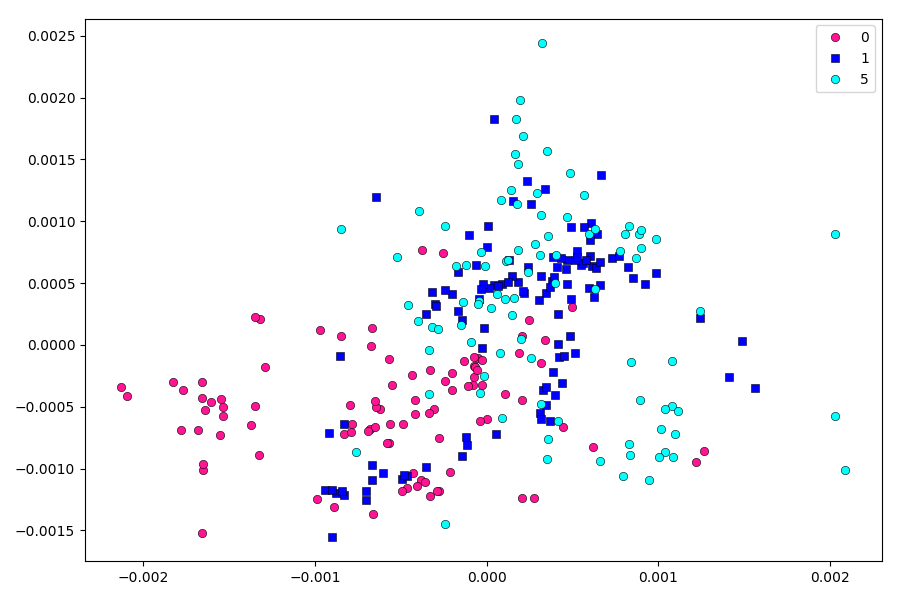
\includegraphics[width=53mm]{pics/tsne_False_iter_20.png}
}
\hspace{0mm}
\subfloat[30 iterations]{
  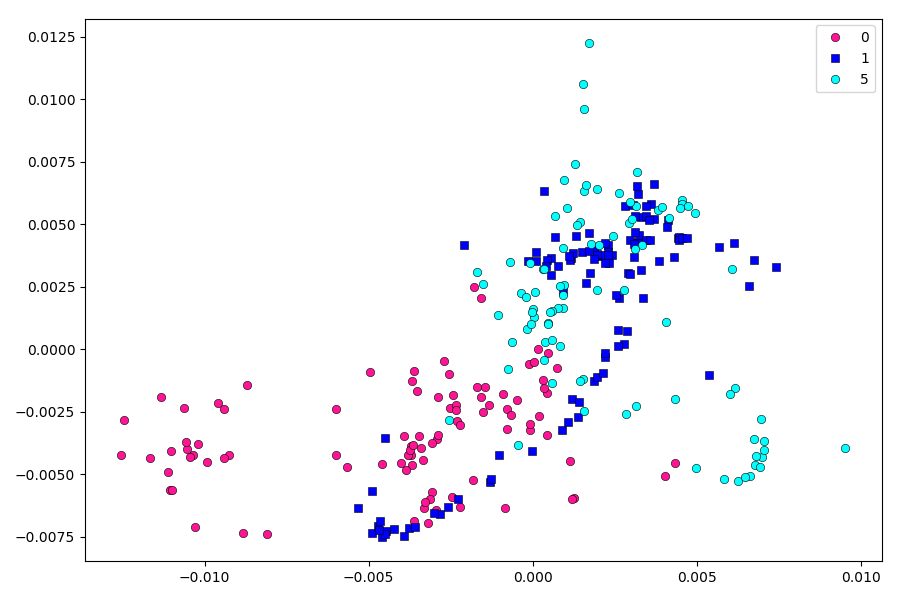
\includegraphics[width=53mm]{pics/tsne_False_iter_30.png}
}
\subfloat[40 iterations]{
  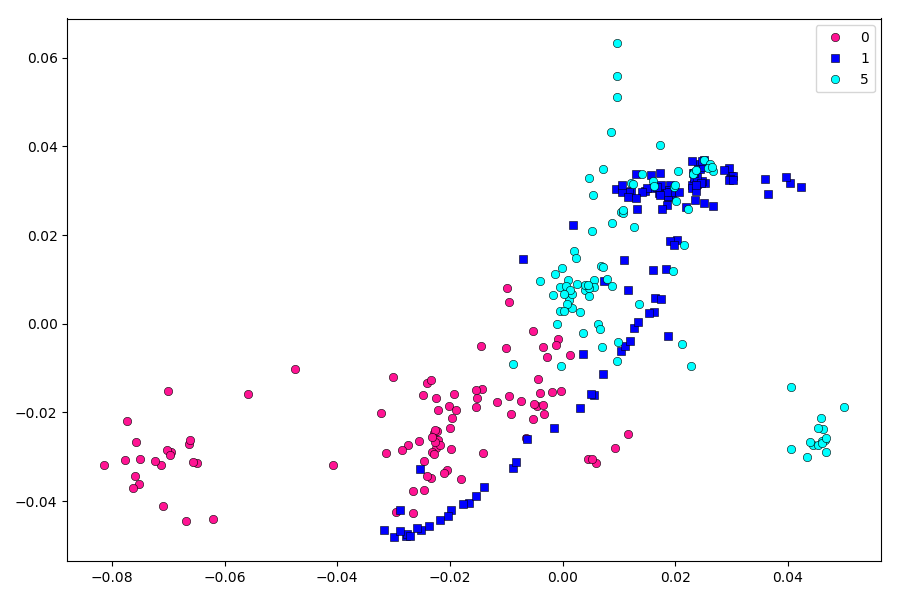
\includegraphics[width=53mm]{pics/tsne_False_iter_40.png}
}
\subfloat[50 iterations]{
  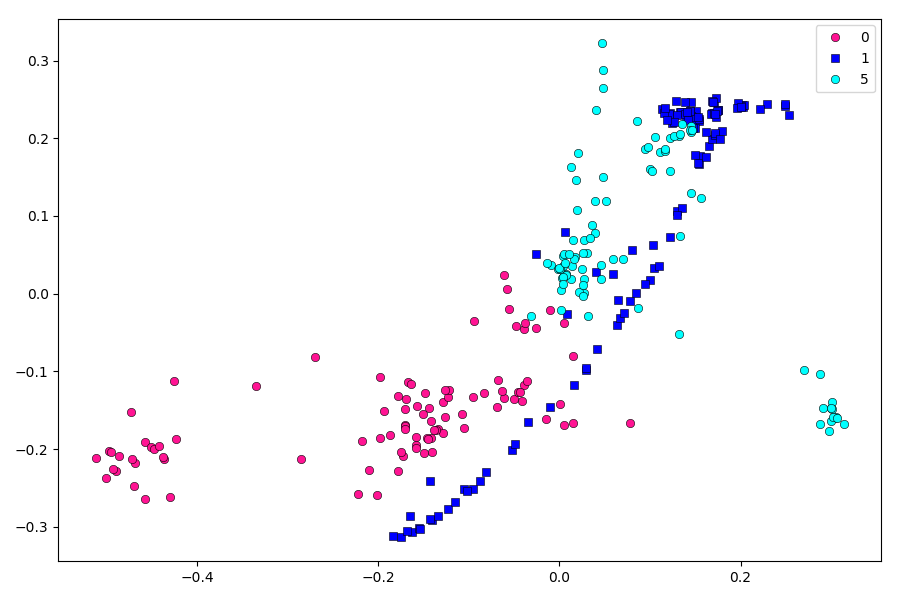
\includegraphics[width=53mm]{pics/tsne_False_iter_50.png}
}
\hspace{0mm}
\subfloat[60 iterations]{
  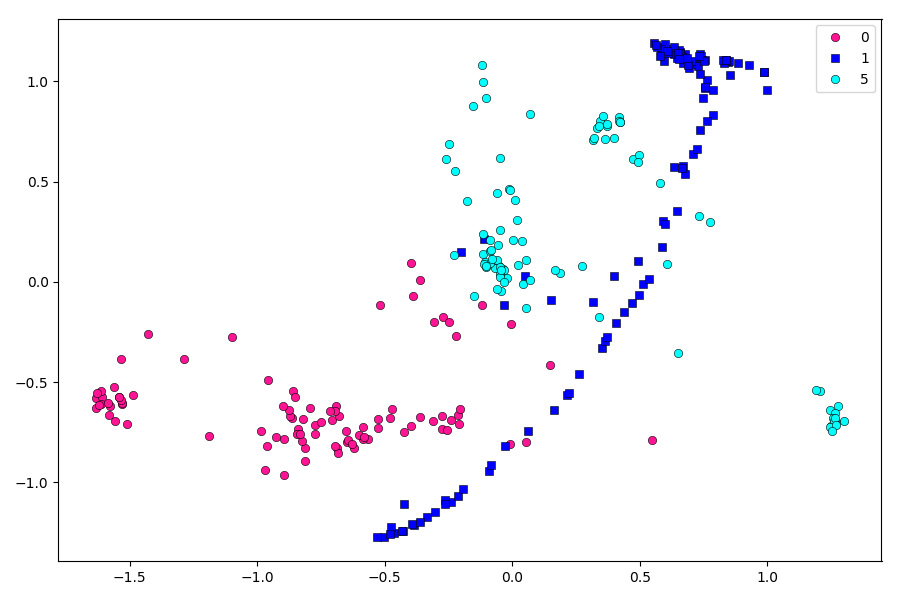
\includegraphics[width=53mm]{pics/tsne_False_iter_60.png}
}
\subfloat[70 iterations]{
  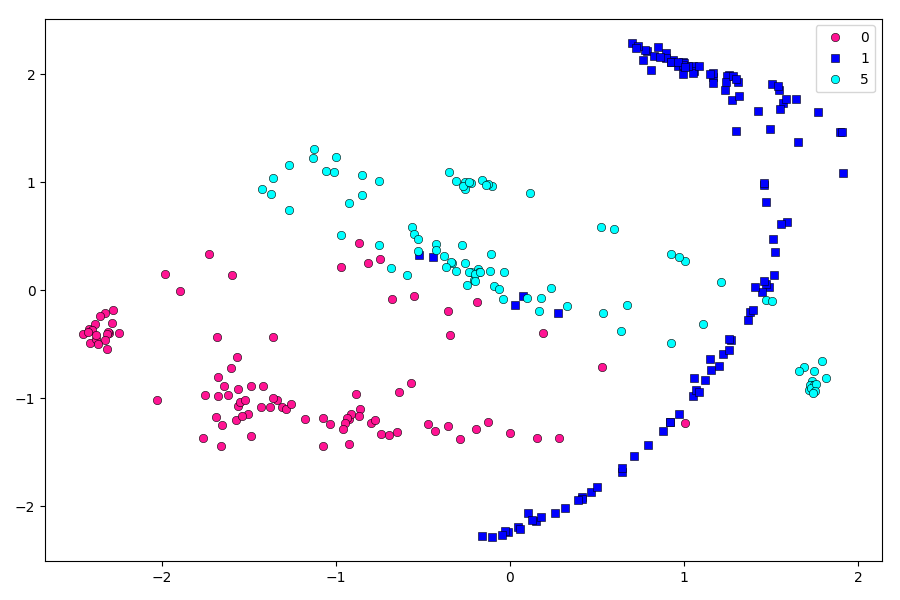
\includegraphics[width=53mm]{pics/tsne_False_iter_70.png}
}
\subfloat[80 iterations]{
  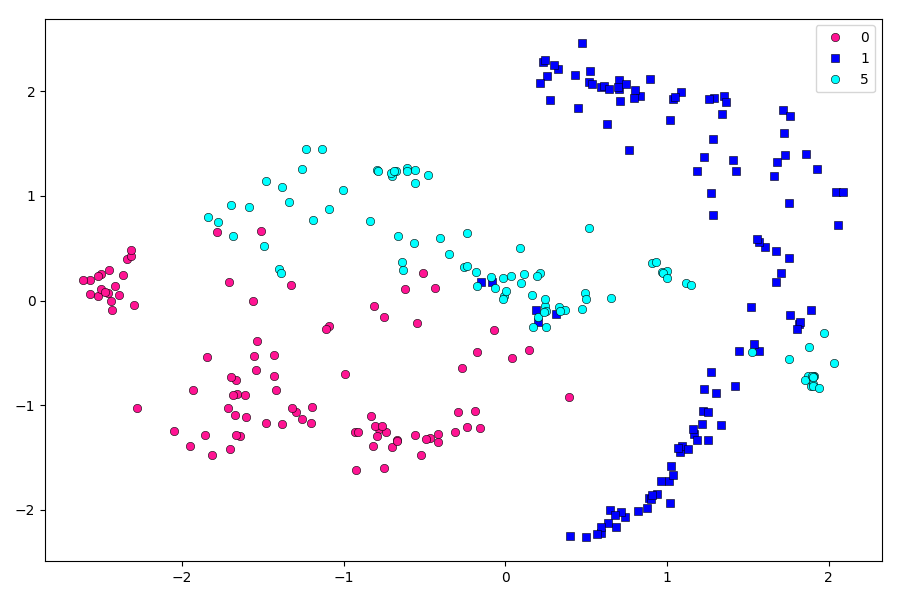
\includegraphics[width=53mm]{pics/tsne_False_iter_80.png}
}
\hspace{0mm}
\subfloat[90 iterations]{
  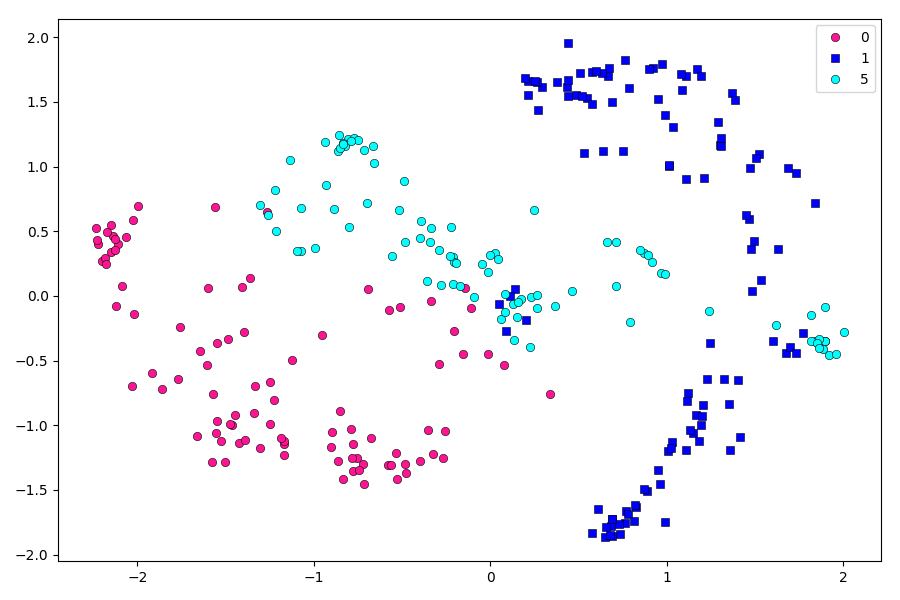
\includegraphics[width=53mm]{pics/tsne_False_iter_90.png}
}
\subfloat[100 iterations]{
  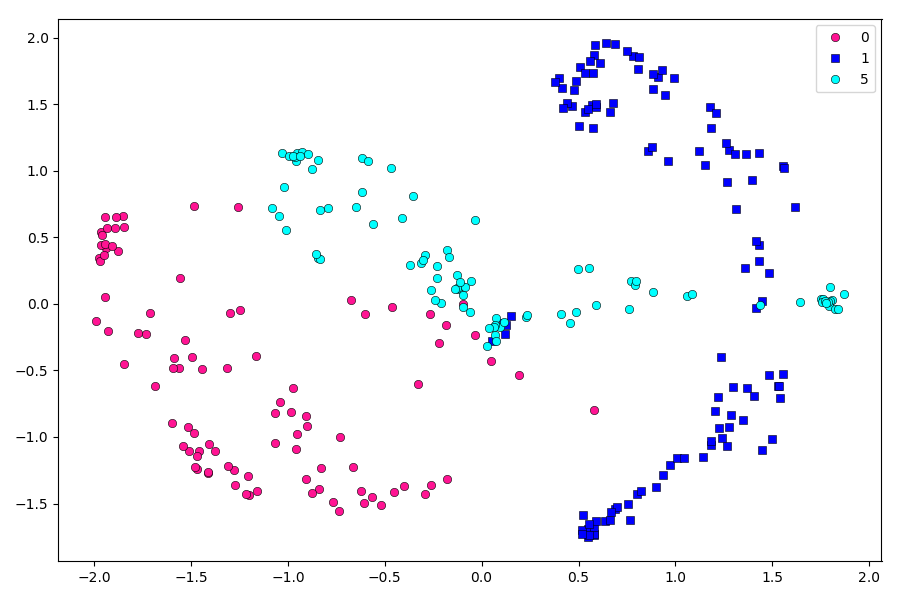
\includegraphics[width=53mm]{pics/tsne_False_iter_100.png}
}
\subfloat[110 iterations]{
  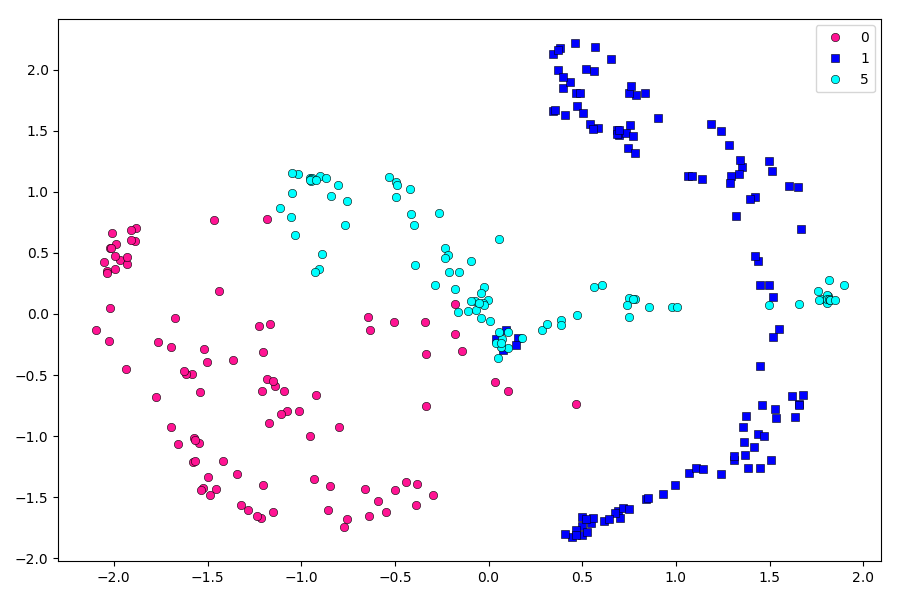
\includegraphics[width=53mm]{pics/tsne_False_iter_110.png}
}
\caption{Results of the SNE applied on the MNIST dataset}
\end{figure}



\end{document}
